
\documentclass{article}

% if you need to pass options to natbib, use, e.g.:
%     \PassOptionsToPackage{numbers, compress}{natbib}
% before loading neurips_2020

% ready for submission
% \usepackage{neurips_2020}

% to compile a preprint version, e.g., for submission to arXiv, add add the
% [preprint] option:
%     \usepackage[preprint]{neurips_2020}

% to compile a camera-ready version, add the [final] option, e.g.:
%     \usepackage[final]{neurips_2020}

% to avoid loading the natbib package, add option nonatbib:
%\usepackage[nonatbib]{neurips_2021}
\usepackage[nonatbib]{neurips_2022}
\usepackage[sort&compress,round]{natbib}
\bibliographystyle{authordate1}

\usepackage{url}            % simple URL typesetting
\usepackage{hyperref}       % hyperlinks
\usepackage[utf8]{inputenc} % allow utf-8 input
\usepackage{xcolor}         % hyperlinks
\usepackage{amsfonts}       % blackboard math symbols
\usepackage{nicefrac}       % compact symbols for 1/2, etc.
\usepackage{microtype}      % microtypography
\usepackage{setspace}
\usepackage{wrapfig}
\usepackage[inline]{enumitem}
\usepackage{caption}     
\usepackage{subcaption}     
\usepackage{float}     
\usepackage{pifont}     
\usepackage{pgfplots}     
%% \usepackage[2-]{pagesel}


\usepackage{amsmath,amssymb,amsthm}
\usepackage{mathtools}

% Math and main text font nonsense
\ifxetex
  \usepackage{fontspec}
  \usepackage{microtype}
  \usepackage{unicode-math}
  \setmathfont{STIXTwoMath-Regular.otf}
  \setmainfont[
    BoldFont={STIXTwoText-Bold.otf}, 
    ItalicFont={STIXTwoText-Italic.otf},
    BoldItalicFont={STIXTwoText-BoldItalic.otf}]{STIXTwoText-Regular.otf}
  %\setmainfont{Times New Roman}
  %\setmathfont{Erewhon-Math.otf}

  %\setmainfont{TeX Gyre Schola}[Scale=0.90] % Text
  % Math: mix of Erewhon and Schola
  %\setmathfont{Erewhon-Math.otf}
  % \setmathfont{TeX Gyre Schola Math}[Scale=0.93,
  %%     range={up/{latin,Latin,num}, it/{latin,Latin,num},
  %%            bfup/{latin,Latin,num}, bfit{latin,Latin,num}}]

  \newcommand{\mathmat}[1]{\symbfup{#1}}
  \newcommand{\mathvec}[1]{\symbfup{#1}}
  \newcommand{\mathvecgreek}[1]{\symbfup{#1}}
  \newcommand{\mathmatgreek}[1]{\symbfup{#1}}

  \newcommand{\mathrv}[1]{\mathsf{#1}}
  \newcommand{\mathrvvec}[1]{\mathbfsf{#1}}
  \newcommand{\mathrvgreek}[1]{\mathsf{#1}}
  \newcommand{\mathrvvecgreek}[1]{\mathbfsf{#1}}
\else
  \usepackage[T1]{fontenc}
  \usepackage[notext,lcgreekalpha]{stix2}
  \usepackage{newtxtext}
  \usepackage{textcomp}

  \newcommand{\mathmat}[1]{\mathbf{#1}}
  \newcommand{\mathvec}[1]{\mathbf{#1}}
  \newcommand{\mathvecgreek}[1]{\mathbf{#1}}
  \newcommand{\mathmatgreek}[1]{\mathbf{#1}}

  \newcommand{\mathrv}[1]{\mathsf{#1}}
  \newcommand{\mathrvvec}[1]{\mathbfsf{#1}}
  \newcommand{\mathrvgreek}[1]{\mathsf{#1}}
  \newcommand{\mathrvvecgreek}[1]{\mathbfsf{#1}}
\fi

\usepackage{booktabs,threeparttable,arydshln}
\usepackage{multirow}
\usepackage{nicematrix}

\usepackage{dsfont}
\usepackage[algo2e, ruled]{algorithm2e}

\usepackage{pgfplots}
\pgfkeys{/pgfplots/tuftelike/.style={
  semithick,
  tick style={major tick length=4pt,semithick,black},
  separate axis lines,
  axis x line*=bottom,
  axis x line shift=2pt,
  xlabel shift=-2pt,
  axis y line*=left,
  axis y line shift=2pt,
  ylabel shift=-2pt}}
  
\usepackage{proof-at-the-end}
\declaretheoremstyle[
    spaceabove=0\topsep,
    spacebelow=0\topsep,
    name={Proposition},
]{propsty}
\declaretheorem[style=propsty]{proposition}

\declaretheoremstyle[
    spaceabove=0\topsep,
    spacebelow=0\topsep,
    name={Theorem},
]{thmsty}
\declaretheorem[style=thmsty]{theorem}

\newtheorem{remark}{\textbf{Remark}}
\newtheorem{lemma}{\textbf{Lemma}}
\newtheorem{assumption}{\textbf{Assumption}}
\newtheorem{condition}{\textbf{Condition}}
%\newtheorem{theorem}{\textbf{Theorem}}
%\newtheorem{proposition}{\textbf{Proposition}}
\newtheorem{definition}{\textbf{Definition}}

\usepackage{mdframed}
\newmdtheoremenv{framedtheorem}{\textbf{Theorem}}
\newmdtheoremenv{framedproposition}{\textbf{Proposition}}
\newmdtheoremenv{framedlemma}{\textbf{Lemma}}

\usepackage{url}
\usepackage{hyperref}
\usepackage[noabbrev, capitalise, nameinlink]{cleveref}

\crefname{assumption}{Assumption}{Assumption}
\crefname{condition}{Condition}{Condition}

\crefname{framedtheorem}{Theorem}{Theorems}
\crefname{framedproposition}{Proposition}{Propositions}
\crefname{framedlemma}{Lemma}{Lemmas}

\makeatletter
\def\adl@drawiv#1#2#3{%
        \hskip.5\tabcolsep
        \xleaders#3{#2.5\@tempdimb #1{1}#2.5\@tempdimb}%
                #2\z@ plus1fil minus1fil\relax
        \hskip.5\tabcolsep}
\newcommand{\cdashlinelr}[1]{%
  \noalign{\vskip\aboverulesep
           \global\let\@dashdrawstore\adl@draw
           \global\let\adl@draw\adl@drawiv}
  \cdashline{#1}
  \noalign{\global\let\adl@draw\@dashdrawstore
           \vskip\belowrulesep}}
\makeatother

\pgfkeys{/prAtEnd/global custom defaults/.style={
    %proof at the end,
    end,
    %normal,
    restate,
    %% text link={\textit{Proof.} See page~\pageref{proof:prAtEnd\pratendcountercurrent} of the \textit{supplementary material}.},
    %text link={\textit{Proof.} The proof is in the \textit{supplementary material}.
    text proof={Proof},
    text link={\textit{Proof.} See the \hyperref[proof:prAtEnd\pratendcountercurrent]{\textit{full proof}} in page~\pageref{proof:prAtEnd\pratendcountercurrent}.}
  }
}

\def\code#1{\texttt{#1}}
\DeclareMathOperator*{\minimize}{minimize}
\DeclareMathOperator*{\maximize}{maximize}
\DeclareMathOperator*{\argmax}{arg\,max}
\DeclareMathOperator*{\argmin}{arg\,min} 

\newcommand*\xbar[1]{%
  \hbox{%
    \vbox{%
      \hrule height 0.6pt % The actual bar
      \kern0.33ex%         % Distance between bar and symbol
      \hbox{%
        \kern-0.1em%      % Shortening on the left side
        \ensuremath{#1}%
        \kern-0.1em%      % Shortening on the right side
      }%
    }%
  }%
} 

\newcommand{\E}[1]{\mathbb{E}\left[\,#1\,\right]}
\newcommand{\Esub}[2]{\mathbb{E}_{#1}\left[\,#2\,\right]}
\newcommand{\V}[1]{\mathbb{V}\left[\,#1\,\right]}
\newcommand{\Vsub}[2]{\mathbb{V}_{#1}\left[\,#2\,\right]}
\newcommand{\Cov}[1]{\mathrm{Cov}\left(\,#1\,\right)}
\newcommand{\Covsub}[2]{\mathrm{Cov}_{#1}\left(\,#2\,\right)}
\newcommand{\Corr}[1]{\mathrm{Corr}\left(\,#1\,\right)}

\newcommand{\Df}[2]{d_{f}(#1\parallel#2)}
\newcommand{\DKL}[2]{d_{\mathrm{KL}}(#1\parallel#2)}
\newcommand{\DChi}[2]{d_{\chi^2}(#1\parallel#2)}
\newcommand{\norm}[1]{{\left\lVert\,#1\,\right\rVert}}
\newcommand{\abs}[1]{{\left|\,#1\,\right|}}
\newcommand{\DTV}[2]{{d_{\mathrm{TV}}\left(#1, #2\right)}}

\newcommand{\vX}{\mathrv{X}}
\newcommand{\vY}{\mathrv{Y}}
\newcommand{\vZ}{\mathrv{Z}}

\newcommand{\va}{\mathvec{a}}
\newcommand{\vb}{\mathvec{b}}
\newcommand{\vc}{\mathvec{c}}
\newcommand{\vd}{\mathvec{d}}
\newcommand{\ve}{\mathvec{e}}
\newcommand{\vf}{\mathvec{f}}
\newcommand{\vg}{\mathvec{g}}
\newcommand{\vh}{\mathvec{h}}
\newcommand{\vi}{\mathvec{i}}
\newcommand{\vj}{\mathvec{j}}
\newcommand{\vk}{\mathvec{k}}
\newcommand{\vl}{\mathvec{l}}
\newcommand{\vm}{\mathvec{m}}
\newcommand{\vn}{\mathvec{n}}
\newcommand{\vo}{\mathvec{o}}
\newcommand{\vp}{\mathvec{p}}
\newcommand{\vq}{\mathvec{q}}
\newcommand{\vr}{\mathvec{r}}
\newcommand{\vs}{\mathvec{s}}
\newcommand{\vt}{\mathvec{t}}
\newcommand{\vu}{\mathvec{u}}
\newcommand{\vv}{\mathvec{v}}
\newcommand{\vw}{\mathvec{w}}
\newcommand{\vx}{\mathvec{x}}
\newcommand{\vy}{\mathvec{y}}
\newcommand{\vz}{\mathvec{z}}
\newcommand{\valpha}{\mathvecgreek{\alpha}}
\newcommand{\veta}{\mathvecgreek{\eta}}
\newcommand{\vmu}{\mathvecgreek{\mu}}
\newcommand{\vtheta}{\mathvecgreek{\theta}}
\newcommand{\vlambda}{\mathvecgreek{\lambda}}
\newcommand{\vxi}{\mathvecgreek{\xi}}

\newcommand{\rva}{\mathrv{a}}
\newcommand{\rvb}{\mathrv{b}}
\newcommand{\rvc}{\mathrv{c}}
\newcommand{\rvd}{\mathrv{d}}
\newcommand{\rve}{\mathrv{e}}
\newcommand{\rvf}{\mathrv{f}}
\newcommand{\rvg}{\mathrv{g}}
\newcommand{\rvh}{\mathrv{h}}
\newcommand{\rvi}{\mathrv{i}}
\newcommand{\rvj}{\mathrv{j}}
\newcommand{\rvk}{\mathrv{k}}
\newcommand{\rvl}{\mathrv{l}}
\newcommand{\rvm}{\mathrv{m}}
\newcommand{\rvn}{\mathrv{n}}
\newcommand{\rvo}{\mathrv{o}}
\newcommand{\rvp}{\mathrv{p}}
\newcommand{\rvq}{\mathrv{q}}
\newcommand{\rvr}{\mathrv{r}}
\newcommand{\rvs}{\mathrv{s}}
\newcommand{\rvt}{\mathrv{t}}
\newcommand{\rvu}{\mathrv{u}}
\newcommand{\rvv}{\mathrv{v}}
\newcommand{\rvw}{\mathrv{w}}
\newcommand{\rvx}{\mathrv{x}}
\newcommand{\rvy}{\mathrv{y}}
\newcommand{\rvz}{\mathrv{z}}
\newcommand{\rvA}{\mathrv{A}}
\newcommand{\rvB}{\mathrv{B}}
\newcommand{\rvC}{\mathrv{C}}
\newcommand{\rvD}{\mathrv{D}}
\newcommand{\rvE}{\mathrv{E}}
\newcommand{\rvF}{\mathrv{F}}
\newcommand{\rvG}{\mathrv{G}}
\newcommand{\rvH}{\mathrv{H}}
\newcommand{\rvI}{\mathrv{I}}
\newcommand{\rvJ}{\mathrv{J}}
\newcommand{\rvK}{\mathrv{K}}
\newcommand{\rvL}{\mathrv{L}}
\newcommand{\rvM}{\mathrv{M}}
\newcommand{\rvN}{\mathrv{N}}
\newcommand{\rvO}{\mathrv{O}}
\newcommand{\rvP}{\mathrv{P}}
\newcommand{\rvQ}{\mathrv{Q}}
\newcommand{\rvR}{\mathrv{R}}
\newcommand{\rvS}{\mathrv{S}}
\newcommand{\rvT}{\mathrv{T}}
\newcommand{\rvU}{\mathrv{U}}
\newcommand{\rvV}{\mathrv{V}}
\newcommand{\rvW}{\mathrv{W}}
\newcommand{\rvX}{\mathrv{X}}
\newcommand{\rvY}{\mathrv{Y}}
\newcommand{\rvZ}{\mathrv{Z}}
\newcommand{\rveta}{\mathrvgreek{\eta}}
\newcommand{\rvlambda}{\mathrvgreek{\lambda}}

\newcommand{\rvva}{\mathrvvec{a}}
\newcommand{\rvvb}{\mathrvvec{b}}
\newcommand{\rvvc}{\mathrvvec{c}}
\newcommand{\rvvd}{\mathrvvec{d}}
\newcommand{\rvve}{\mathrvvec{e}}
\newcommand{\rvvf}{\mathrvvec{f}}
\newcommand{\rvvg}{\mathrvvec{g}}
\newcommand{\rvvh}{\mathrvvec{h}}
\newcommand{\rvvi}{\mathrvvec{i}}
\newcommand{\rvvj}{\mathrvvec{j}}
\newcommand{\rvvk}{\mathrvvec{k}}
\newcommand{\rvvl}{\mathrvvec{l}}
\newcommand{\rvvm}{\mathrvvec{m}}
\newcommand{\rvvn}{\mathrvvec{n}}
\newcommand{\rvvo}{\mathrvvec{o}}
\newcommand{\rvvp}{\mathrvvec{p}}
\newcommand{\rvvq}{\mathrvvec{q}}
\newcommand{\rvvr}{\mathrvvec{r}}
\newcommand{\rvvs}{\mathrvvec{s}}
\newcommand{\rvvt}{\mathrvvec{t}}
\newcommand{\rvvu}{\mathrvvec{u}}
\newcommand{\rvvv}{\mathrvvec{v}}
\newcommand{\rvvw}{\mathrvvec{w}}
\newcommand{\rvvx}{\mathrvvec{x}}
\newcommand{\rvvy}{\mathrvvec{y}}
\newcommand{\rvvz}{\mathrvvec{z}}
\newcommand{\rvvlambda}{\mathrvvecgreek{\lambda}}
\newcommand{\rvveta}{\mathrvvecgreek{\eta}}

\newcommand{\mA}{\mathmat{A}}
\newcommand{\mB}{\mathmat{B}}
\newcommand{\mC}{\mathmat{C}}
\newcommand{\mD}{\mathmat{D}}
\newcommand{\mE}{\mathmat{E}}
\newcommand{\mF}{\mathmat{F}}
\newcommand{\mG}{\mathmat{G}}
\newcommand{\mH}{\mathmat{H}}
\newcommand{\mI}{\mathmat{I}}
\newcommand{\mJ}{\mathmat{J}}
\newcommand{\mK}{\mathmat{K}}
\newcommand{\mL}{\mathmat{L}}
\newcommand{\mM}{\mathmat{M}}
\newcommand{\mN}{\mathmat{N}}
\newcommand{\mO}{\mathmat{O}}
\newcommand{\mP}{\mathmat{P}}
\newcommand{\mQ}{\mathmat{Q}}
\newcommand{\mR}{\mathmat{R}}
\newcommand{\mS}{\mathmat{S}}
\newcommand{\mT}{\mathmat{T}}
\newcommand{\mU}{\mathmat{U}}
\newcommand{\mV}{\mathmat{V}}
\newcommand{\mW}{\mathmat{W}}
\newcommand{\mX}{\mathmat{X}}
\newcommand{\mY}{\mathmat{Y}}
\newcommand{\mZ}{\mathmat{Z}}
\newcommand{\mSigma}{\mathmatgreek{\Sigma}}

\newcommand{\iprod}[2]{\left\langle #1, #2 \right\rangle}
\newcommand{\ind}[1]{\mathds{1}_{#1}}


\allowdisplaybreaks

%% Tikz corner
\usepackage{tikz}
\usepackage{pgf}
\usepackage{pgfplots}
\usepackage{pgfplotstable}
\pgfplotsset{compat=1.18}
\usetikzlibrary{patterns}
\usetikzlibrary{fit, calc}
\usetikzlibrary{pgfplots.groupplots}
\usepgfplotslibrary{fillbetween}
\usepgfplotslibrary{groupplots}
\usepgfplotslibrary{statistics}
\usepgfplotslibrary{external} 

\definecolor{darkgrey}{HTML}{3E3E3E}

\usepackage{pifont}
\usepackage{xcolor}
\newcommand{\cmark}{\textcolor{green!80!black}{\ding{51}}}
\newcommand{\xmark}{\textcolor{red}{\ding{55}}}
\newcommand{\jrg}[1]{\textcolor{red}{[Jake: #1]}}
\newcommand{\krk}[1]{\textcolor{blue}{#1}}

\tikzset{external/system call={xelatex -shell-escape -halt-on-error -interaction=batchmode -jobname "\image" "\texsource"}}
\tikzexternalize
\tikzexternaldisable

\title{Markov Chain Score Ascent: \\ A Unifying Framework of \\ Variational Inference with Markovian Gradients}

% The \author macro works with any number of authors. There are two commands
% used to separate the names and addresses of multiple authors: \And and \AND.
%
% Using \And between authors leaves it to LaTeX to determine where to break the
% lines. Using \AND forces a line break at that point. So, if LaTeX puts 3 of 4
% authors names on the first line, and the last on the second line, try using
% \AND instead of \And before the third author name.

\author{%
%   Kyurae Kim, Jisu Oh, Hongseok Kim \\
%   Sogang University \\
%   \texttt{\{msca8h, \}@sogang.ac.kr} \\
}

%% \author{%
%%   David S.~Hippocampus\thanks{Use footnote for providing further information
%%     about author (webpage, alternative address)---\emph{not} for acknowledging
%%     funding agencies.} \\
%%   Department of Computer Science\\
%%   Cranberry-Lemon University\\
%%   Pittsburgh, PA 15213 \\
%%   \texttt{hippo@cs.cranberry-lemon.edu} \\
%%   % examples of more authors
%%   % \And
%%   % Coauthor \\
%%   % Affiliation \\
%%   % Address \\
%%   % \texttt{email} \\
%%   % \AND
%%   % Coauthor \\
%%   % Affiliation \\
%%   % Address \\
%%   % \texttt{email} \\
%%   % \And
%%   % Coauthor \\
%%   % Affiliation \\
%%   % Address \\
%%   % \texttt{email} \\
%%   % \And
%%   % Coauthor \\
%%   % Affiliation \\
%%   % Address \\
%%   % \texttt{email} \\
%% }

\begin{document}

\maketitle

\begin{abstract}
  
Recently, variational inference methods that minimize the inclusive Kullback-Leibler (KL) divergence using Markov-chain Monte Carlo (MCMC) have been developed.
These methods perform stochastic gradient descent by obtaining noisy estimates of the score function using MCMC.
%While conceptually similar, one uses a single Markov-chain state from the conditional importance sampling (CIS) kernel while the other uses multiple states from the independent Metropolis-Hastings (IMH).
%So far, multiple ways to operate the Markov-chains have proposed, but it is unclear which results in better VI performance.
In this paper, we compare three different ways to operate Markov-chains for VI, and compare the performance of different schemes.
In particular, we propose the parallel state estimator, which averages a single state of multiple parallel Markov-chains.
Compared to previously used MCMC based score climbing schemes, this estimator has lower variance enabling faster convergence.
Our experiments show that, when using our proposed scheme, inclusive KL divergence minimization is competitive against evidence lower bound minimization.
%Our results motivate the use of the inclusive KL divergence for VI.

%%% Local Variables:
%%% TeX-master: "master"
%%% End:

\end{abstract}


\section{Introduction}
Given an observed data \(\vx\) and a latent variable \(\vz\), Bayesian inference aims to analyze the posterior distribution \(p\,(\vz\,|\,\vx)\) given an unnormalized joint density \(p\,(\vz,\,\vx)\) where the relationship is given by Bayes' rule such that \(p\,(\vz\,|\,\vx) = {p\,(\vz,\,\vx)}/{p\,(\vx)} \propto p\,(\vz,\,\vx)\).
For clarity, we will denote the posterior distribution as \(\pi\left(\vz\right) = p\,(\vz\mid\vx)\).
Instead of working directly with the target distribution \(\pi\), variational inference (VI,~\citealt{blei_variational_2017}) searches for a variational approximation \(q_{\lambda}(\vz)\) that is similar to \(\pi\) according to a discrepancy measure \(D\,(\pi,\, q_{\vlambda})\).

Naturally, choosing a discrepancy measure is critical to the problem.
This fact had led to a quest for suitable divergence measures~\citep{pmlr-v37-salimans15, NIPS2016_7750ca35, NIPS2017_35464c84, NEURIPS2018_1cd138d0, pmlr-v97-ruiz19a}.
So far, the exclusive KL divergence \(\DKL{q_{\lambda}}{\pi}\) (or reverse KL divergence) has been used ``exclusively'' among various discrepancy measures.
This is partly because the exclusive KL is defined as an average over \(q_{\lambda}(\vz)\), which can be estimated efficiently.
By contrast, the inclusive KL is defined as
%
{\small
\vspace{-0.05in}
\begin{align}
  %% \DKL{p}{q_{\lambda}} = \int p\,(\vz\mid\vx) \log\big(\, p\,(\vz\mid\vx)/q_{\lambda}(\vz) \,\big)\,d\vz
  %% = \Esub{p(\vz\mid\vx)}{\log\big(\, p\,(\vz\mid\vx)/q_{\lambda}(\vz) \,\big) } \label{eq:klpq}
  \DKL{\pi}{q_{\lambda}}
  = \int \pi\,(\vz) \log \frac{\pi\left(\vz\right)}{\,q_{\lambda}(\vz)} \,d\vz
  = \Esub{\pi}{\log \frac{\pi\left(\vz\right)}{\,q_{\lambda}(\vz)} } \label{eq:klpq}
\end{align}
%\vspace{-0.05in}
}%
%
where the average is taken over \(\pi\). 
This is a chicken-and-egg problem as our goal is to obtain \(\pi\) in the first place.
Despite this challenge, minimizing~\eqref{eq:klpq} has drawn the attention of researchers because it is believed to result in favorable properties~\citep{minka2005divergence, mackay_local_2001}.

For minimizing the inclusive KL divergence,~\citet{NEURIPS2020_b2070693} and~\citet{pmlr-v124-ou20a} have recently proposed  methods that perform stochastic gradient descent (SGD,~\citealt{robbins_stochastic_1951}) with the score function estimated using Markov-chain Monte Carlo (MCMC).
These MCMC score climbing schemes operate a Markov chain in conjunction with the VI optimizer.
In addition, within the MCMC kernel, they both use Metropolis-Hastings proposals generated from the variational approximation \(\vz^* \sim q_{\vlambda}\left(\cdot\right)\).
The MCMC kernel itself benefits from VI, enjoying better proposals over time without the need for computationally expensive proposals as in Hamiltonian Monte Carlo~\citep{duane_hybrid_1987, neal_mcmc_2011, betancourt_conceptual_2017}.
Also, in terms of computational cost, score climbing is efficient compared to other divergences since we do not need to differentiate through the likelihood.

While the convergence of score climbing VI has been established by~\citet{NEURIPS2020_b2070693, gu_stochastic_1998}, the practical performance implications of the design choices have yet to be understood.
For example, the methods by~\citeauthor{NEURIPS2020_b2070693} and~\citet{pmlr-v124-ou20a} are conceptually similar, but they utilize MCMC kernels in different ways.
At each SGD iteration, for estimating the score function, \citeauthor{NEURIPS2020_b2070693} use a single sample generated from a relatively expansive MCMC kernel, while~\citeauthor{pmlr-v124-ou20a} average multiple samples generated from a cheaper MCMC kernel.
We call the former scheme the \textit{single state estimator} and the later the \textit{sequential state estimator}.
Given the two options, it is natural to ask, ``which is better? An estimator with multiple cheap samples? or one with a single expensive sample?''.

This paper proposes a third scheme, the \textit{parallel state estimator}.
The parallel state estimator operates \(N\) parallel Markov-chains parallel, where only a single state transition is performed on each chain.
The variance of this estimator linearly decreases with the computational budget \(N\), unlike the single and sequential state estimators.
However, according to the traditional MCMC intuition, this improvement would come at the cost of increased bias.
In the example in~\cref{section:motivation}, we show that this intuition can be wrong in the score climbing setting, occasionally resulting in \textit{lower} bias than the longer Markov-chains of the sequential state estimator.
%This is because the much lower variance of the parallel estimator results in the VI procedure converging faster compared to other estimators.

To explain the unintuitive performance benefit of the parallel state estimator, we theoretically analyze the variance of the considered estimators.
Then, we show that the KL objective bounds the bias of the parallel state estimator, which means bias decreases as VI converges.
The low variance of the parallel state estimator results in fast convergence and thus a fast decrease in bias.
This suggests that, given a similar computational budget, the parallel state estimator is overall better than the alternative estimators.
We also provide experimental evidence on general Bayesian inference problems.
Also, our experiments show that score climbing VI with the parallel state estimator is competitive against evidence lower-bound (ELBO) maximization.
We further discuss this result in relation with the conclusions of~\citet{dhaka_challenges_2021} in~\cref{section:discussion}.

%% generated by the conditional importance sampling (CIS,~\citealt{NEURIPS2020_b2070693, andrieu_particle_2010, andrieu_uniform_2018}) kernel, which uses \(N\) samples from \(q_{\vlambda}(\cdot)\) per transition.
%% \citeauthor{pmlr-v124-ou20a}, on the other hand, use multiple sequentially generated states from independent Metropolis-Hastings (IMH,~\citealt[Algorithm 25]{hastings_monte_1970}), which only uses 1 sample from \(q_{\vlambda}(\cdot)\).
%% Therfore, \citeauthor{pmlr-v124-ou20a} use multiple cheaply generated samples, while \citeauthor{NEURIPS2020_b2070693} use a single expensively generated samples.

%Finally, some interesting connections with adaptive MCMC methods~\citep{10.1007/s11222-008-9110-y} are discussed.

%\vspace{-0.05in}
%\paragraph{Contribution Summary}
%\vspace{-0.2in}
\begin{itemize}[noitemsep]
\item[\ding{228}] We propose the parallel state estimator for variational score climbing (\textbf{\cref{section:overview}}).
\item[\ding{228}] The parallel state estimator achieves lower variance than the sequential~\citep{pmlr-v124-ou20a} and single state esimators~\citep{NEURIPS2020_b2070693} (\textbf{\cref{section:var}}).
\item[\ding{228}] We show that the parallel state does not necessarily result in higher bias, making it the best option overall (\textbf{\cref{section:bias}}).
\item[\ding{228}] We experimentally compare the VI performance of the considered MCMC estimators on general Bayesian inference benchmarks (\textbf{\cref{section:eval}}).
\end{itemize}
\vspace{-0.05in}
%\item We discuss connections with adaptive IMH methods (\textbf{\cref{section:related}}).
%\end{enumerate*}

%%% Local Variables:
%%% TeX-master: "master"
%%% End:


\vspace{-0.1in}
\section{Background}
\subsection{Variational Inference with Stochastic Gradients}\label{section:ivi_previous}
The goal of VI is to find the optimal variational parameter \(\vlambda\) identifying \(q_{\vlambda} \in \mathcal{Q}\) that minimizes some discrepancy measure \(D\left(\pi, q_{\vlambda}\right)\).
A typical way to perform VI is to use stochastic gradient descent (SGD,~\citealt{robbins_stochastic_1951}), provided that gradient estimates of the optimization target \(\vg\,(\vlambda)\) are available.
In this case, SGD is performed by repeating the update
%\vspace{-0.05in}
{%\small
\begin{align*}
  \vlambda_{t} = \vlambda_{t-1} + \gamma_{t} \, \vg\left(\vlambda_{t-1}\right)
\end{align*}
}
where \(\gamma_1, \ldots, \gamma_T\) is a step-size schedule following the conditions of~\citet{robbins_stochastic_1951, bottou_online_1999}.
In the case of inclusive KL divergence minimization, \(\vg\) estimates
%
{%\small
\begin{align*}
  \nabla_{\vlambda} \DKL{\pi}{q\left(\cdot; \lambda\right)}
  = -\Esub{\pi}{ \vs\,(\vlambda; \rvvz) } 
  \approx \vg\left(\vlambda\right)
\end{align*}
}%
%\vspace{-0.05in}
%
where \(\vs\,(\vlambda;\vz) = \nabla_{\vlambda} \log q\,(\vz; \vlambda)\) is known as the \textit{score gradient}.

Since the optimization target is equivalent to ascending towards the direction of the score, \citet{NEURIPS2020_b2070693} coined the term score climbing.
To better conform to the optimization literature, we instead call this approach \textit{score ascent} (as in gradient ascent).

%\vspace{-0.05in}
%% \subsection{Estimating the Score with Importance Sampling}\label{section:is}
%% When it is easy to sample from the variational approximation \(q_{\lambda}(\vz)\), one can use importance sampling (IS, \citealt{robert_monte_2004}) for estimating the score following
%% %\vspace{-0.05in}
%% {%\small
%% \begin{align*}
%%   \Esub{\pi}{ \vs\,(\vlambda;\rvvz) } 
%%   \propto Z\,\Esub{\pi}{ \vs\,(\vlambda; \rvvz) } %\label{eq:is_est} \\
%%   \approx \frac{1}{N} \sum^{N}_{i=1} \widetilde{w}\,(\vz^{(i)}) \, \vs\,(\vlambda; \vz^{(i)}) 
%%   \triangleq \vg_{IS}(\vlambda)
%% \end{align*}
%% }%
%% %\vspace{-0.05in}
%% where \(\widetilde{w}\,(\vz) = p\,(\vz,\vx) / q_{\vlambda}(\vz)\) is known as the unnormalized importance weight, \(Z\) is the marginal \(p\left(\vx\right) = \int p\left(\vx, \vz\right) \, d\vz\), and \(\vz^{(1)},\, \ldots,\, \vz^{(N)}\) are \(N\) independent samples from \(q_{\vlambda}(\vz)\).
%% This scheme is equivalent to adaptive IS methods~\citep{bugallo_adaptive_2017} since the IS proposal \(q_{\vlambda}(\vz)\) is iteratively optimized based on the current samples.
%% Although IS is unbiased, it is numerically unstable because of \(Z\). %in \cref{eq:is_est}.
%% A more stable alternative is to use the normalized weight, which results in the self-normalized IS (SNIS) approximation.
%% Unfortunately, SNIS still fails to converge even on moderate dimensional objectives and unlike IS, it is no longer unbiased~\citep{robert_monte_2004}.

\subsection{Markov Chain Gradient Descent}\label{section:mcgd}
Markov chain gradient descent (MCGD, \citealt{duchi_ergodic_2012, NEURIPS2018_1371bcce}) is a family of algorithm that minimize (or maximize) a function \(f\) defined as \(f\left(\vlambda\right) = \int f\left(\vlambda, \veta\right) \, \Pi\left(d\veta\right)\) where \(\Pi\left(d\veta\right)\) is a probability measure.
MCGD repeats the steps 
{%\small
\begin{align}
  \vlambda_{t+1}    = \vlambda_{t} + \gamma_t \, \vg\left(\vlambda_t, \veta_{t}\right),\quad 
  \rvveta_{t}  \sim P_{\vlambda_{t-1}}\left( \veta_{t-1}, \cdot \right)\label{eq:mcgd}
\end{align}
}%
where \(P_{\vlambda_{t-1}}\) is a \(\Pi\)-invariant Markov chain kernel that could depend on \(\vlambda_{t-1}\).
Unlike vanilla SGD where the gradient noise is assumed to be \textit{i.i.d.} and unbiased, the gradient noise is now Markovian and non-asymptotically biased.
Therefore, a different analysis methodology is needed to analyze the non-asymptotic convergence, as done by~\citep{duchi_ergodic_2012, NEURIPS2018_1371bcce, pmlr-v99-karimi19a, doan_finitetime_2020, doan_convergence_2020, Xiong_Xu_Liang_Zhang_2021, debavelaere_convergence_2021}.
The MCGD setting encompasses an extensive range of problems, including distributed optimization~\citep{ram_incremental_2009}, reinforcement learning~\citep{tadic_asymptotic_2017, doan_convergence_2020, Xiong_Xu_Liang_Zhang_2021}, and expectation-minimization~\citep{pmlr-v99-karimi19a}, to name a few.
This paper shows that the MCSA setting is part of the MCGD framework, which provides some practical insights into MSCA.

%%% Local Variables:
%%% TeX-master: "master"
%%% End:


%\vspace{-0.05in}
\section{Chain Wielding Strategies for Markov-chain Monte Carlo Estimators in Inclusive Variational Inference}
\vspace{-0.05in}
\subsection{Overview of Prevoius Estimation Strategies}\label{section:jsa_msc}
%
\vspace{-0.05in}

\paragraph{Overview}
Recently,~\citeauthor{NEURIPS2020_b2070693} and~\citeauthor{pmlr-v124-ou20a} proposed two similar but independent methods for performing inclusive variational inference.
Both methods estimate the score gradient by operating a Markov-chain in parallel with the VI optimization sequence.
Also, they both use MCMC kernels that can effectively used the variational approximation \(q_{\vlambda_t}(\vz)\).
Because of this, compared to previous VI approaches~\citep{pmlr-v97-ruiz19a, pmlr-v70-hoffman17a} that use expensive MCMC kernels such as Hamiltonian Monte Carlo, both methods are computationally efficient. 

\vspace{-0.05in}
\paragraph{Markovian Score Climbing and the Single State Estimator}
In Markovian score climbing (MSC), \citep{NEURIPS2020_b2070693} estimate the score gradient by performing an MCMC iteration and update the parameters such that
\vspace{-0.05in}
\begin{align}
  &\vz_t \sim K\left(\vz_{t-1}, \cdot \right) &g_{\text{single-CIS}}(\vlambda) = s\,(\vz_t; \vlambda)
\end{align}
where \(K\left(\vz_{t-1}, \cdot\right)\) is a MCMC kernel leaving \(p\,(\vz\mid\vx)\) invariant and \(g_{\text{single}}\left(\vlambda\right)\) denotes the score estimator.
For \(K\left(\vz_{t-1}, \cdot\right)\), they propose a new type of kernel inspired by particle MCMC~\cite{andrieu_particle_2010}, the conditional importance sampling (CIS) kernel.
Since the estimator uses \textit{a single state} created by the CIS kernel, we call it the single state estimator with the CIS kernel (single-CIS).
The CIS kernel internally uses \(N\) samples from the \(q_{\vlambda}(\vz)\).
Thus, when compared to MCMC kernels that only use a single sample from \(q_{\vlambda}(\vz)\), it is \(N\) times more expensive, but hopefully, statistically superior.
Unfortunately, we will show that this is not the case.

\vspace{-0.05in}
\paragraph{Joint Stochastic Approximation and the Sequential State Estimator}
On the other hand, at each SGD iteration \(t\),~\citep{pmlr-v124-ou20a} perform \(N\) sequential Markov-chain transitions and use the average of the intermediate states for estimation.
That is, for the index \(i \in \{1, \ldots, N\}\),
\vspace{-0.05in}
\begin{align}
  &\vz_{T+i} \sim K^i\left(\vz_{T}, \cdot \right) &g_{\text{seq.-IMH}}(\vlambda) = \frac{1}{N} \sum_{i=1}^N s\,(\vz_{T+i}; \vlambda)
\end{align}
where \(\vz_T\) is the last Markov-chain state of the previous SGD iteration.
For the MCMC kernel, they use the classic independent Metropolis-Hastings (IMH,~\citealt[Algorithm 25]{robert_monte_2004}~\citealt{hastings_monte_1970}) algorithm, which uses only a single sample from \(q_{\vlambda}(\vz)\).
Therefore, the cost of \(N\) state transitions with IMH is similar to the cost of a single transition with CIS.
Since the estimator uses sequential states, we call it the sequential state esimator with the IMH kernel (seq.-IMH)

\vspace{-0.05in}
\paragraph{Additional  Notes on JSA}
Before preoceeding, we acknowledge that the setup of~\citet{pmlr-v124-ou20a} is slightly different than what we described.
Their MCMC kernel leave \(p\left(\vz_j\mid\vx_j \right)\) invariant for a single datapoint \(\vx_j\), which is only possible when the datapoints are independently, identically distributed (\textit{iid}) under the probabilistic model.
We interpret their method more generally and assume that we only have a kernel that can leave \(p\left(\vz\mid\vx \right)\) invariant.

\subsection{Overview of Markov-Chain Monte Carlo Score Estimation Strategies}\label{section:overview}

\begin{figure*}
  \vspace{-0.4in}
    \centering
    \begin{subfigure}[b]{0.25\textwidth}
        \centering
        \includegraphics[scale=0.25]{figures/diagram_1.png}
        \caption{Single state estimator}\label{fig:single}
    \end{subfigure}
    \begin{subfigure}[b]{0.35\textwidth}
        \centering
        \includegraphics[scale=0.25]{figures/diagram_2.png}
        \caption{Sequential state estimator}\label{fig:seq}
    \end{subfigure}
    \begin{subfigure}[b]{0.3\textwidth}
        \centering
        \includegraphics[scale=0.25]{figures/diagram_3.png}
        \caption{Parallel state estimator}\label{fig:par}
    \end{subfigure}
    \caption{Visualization of different ways of combining MCMC with stochastic approximation variational inference.
    The index \(t\) denotes the stochastic approximation iteration.
    The dark circles denote the MCMC samples used for estimating the score gradient at \(t=2\).
    }\label{fig:overview}
\end{figure*}

\vspace{-0.05in}
\paragraph{Single State and Sequential State Estimators}
The two different MCMC estimators used in MSC and JSA represent two different ways of using a fixed computational budget.
The former uses a computationally expensive, but hopefully statistically superior, MCMC kernel with less samples, while the latter uses a cheaper MCMC kernel with more samples.
Illustrations of the two schemes are shown in~\cref{fig:single,fig:seq}.
Detailed pseudocodes of the considered schemes are provided in the \textit{supplementary material}.

\vspace{-0.05in}
\paragraph{Parallel State Estimator}
In this work, we will add a new scheme into the mix: the parallel state estimator.
Similarly with the sequential state estimator, we use the cheaper IMH kernel, but instead of applying the MCMC kernel \(N\) times to a single chain, we apply the MCMC kernel a single time to \(N\) \textit{parallel Markov-chains}.
That is, for each Markov-chain \(i \in \{1, \ldots, N\}\),
%
\vspace{-0.05in}
\begin{align}
  &\vz_{t}^{(i)} \sim K\big(\vz_{t-1}^{(i)}, \cdot \big) &g_{\text{par.-IMH}}(\vlambda) = \frac{1}{N} \sum_{i=1}^N s\,(\vz_{t}^{(i)}; \vlambda)
\end{align}
%
where \(\vz_{t-1}^{(i)}\) is the state of the \(i\)th chain at the previous SGD step.
Computationally speaking, we are still applying \(K\big(\vz_{t-1}^{(i)}\big)\) \(N\) times in total, so the cost is similar to the sequential state estimator.
However, the Markov-chain are \(N\) times shorter, which, in a traditional MCMC view, might seem to result in worse statistical performance.
An illustration of the parallel state estimator is shown in~\cref{fig:par}

%

% Second version of table, with booktabs.
\begin{table*}
\centering
\caption{Computational Cost of Markov-chain Schemes}\label{table:cost}
\setlength{\tabcolsep}{2pt}
  \begin{threeparttable}
\begin{tabular}{lccccc}\toprule
& \multicolumn{3}{c}{\footnotesize Estimation} & \multicolumn{2}{c}{\footnotesize Stochastic gradient} \\
\cmidrule(lr){2-4}\cmidrule(lr){5-6}
  & \(\footnotesize p\left( \vz, \vx \right)\)
  & \(\footnotesize q_{\vlambda}(\vz)\)
  & \(\footnotesize q_{\vlambda}(\vz)\)
  & \(\footnotesize p\left( \vz, \vx \right)\)
  & \(\footnotesize q_{\vlambda}(\vz)\)
  \\
  & {\footnotesize\# Eval.  }
  & {\footnotesize\# Eval.  }
  & {\footnotesize\# Samples}
  & {\footnotesize\# Grad.  }
  & {\footnotesize\# Grad.  }
%
\\\midrule
%
{\footnotesize
ADVI
}
& \(0\)
& \(0\)
& \(N\)
& \(N\)
& \(0\)
\\\arrayrulecolor{black!30}\midrule
%
{\footnotesize
Single state estimator with CIS
}
& \(N-1\)
& \(N\)
& \(N-1\)
& \(0\)
& \(1\)\tnote{1}\;\;{\footnotesize or}\;\(N\)\tnote{2}
\\
%
{\footnotesize
Sequential state estimator with IMH
}
& \(N\)
& \(N\)
& \(N\)
& \(0\)
& \(N\)
\\
%
{\footnotesize
Parallel state estimator with IMH
}
& \(N\)
& \(N\)
& \(N\)
& \(0\)
& \(N\)
\\\bottomrule
\end{tabular}
  \begin{tablenotes}
    \item[*]{\footnotesize \(N\) is the number of samples used in each method}.
    \item[1]{\footnotesize Vanilla CIS kernel}.
    \item[2]{\footnotesize Rao-Blackwellized CIS kernel}.
  \end{tablenotes}
  \end{threeparttable}
\end{table*}

%
\paragraph{Computational Cost}
The three scheme using the CIS kernel and the IMH kernel can have different computational cost depending on the parameter \(N\).
The computational costs of each scemes are organized in~\cref{table:cost}.
In the CIS kernel, \(N\) controls the number of internal proposals sampled from \(q_{\vlambda}(\vz)\).
In the sequential and parallel state estimators, the IMH kernel only uses a single sample from \(q_{\vlambda}(\vz)\), but applies the kernel \(N\) times.
When estimating the score, the single state estimator computes \(\nabla_{\vlambda} q_{\vlambda}(\vz)\) only once, while for the sequential and parallel state estimators compute it \(N\) times.
However,~\cite{NEURIPS2020_b2070693} also discuss a Rao-Blackwellized version of the CIS kernel, which also computes the gradient \(N\) times.

\subsection{Theoretical Analysis}

\textcolor{red}{
  \paragraph{Boundedness Assumption}
Since we derive our bounds on the bias from the total-variation distance, our results assume that the score function is bounded.
That is, \(\norm{\nabla_{\vlambda} \log q_{\vlambda}(\vz)} < L\) for any \(\vlambda\).
This boundedness assumption is reasonable since theoretical guarentees of SGD often assume Lipschitz-continuity of the gradients, from which boundedness follow as a consequence.
}


\begin{theoremEnd}{theorem}\label{thm:bias_seq}
  Assuming \(w^* = \sup_{\vz} \nicefrac{p\left(\vz\mid\vx\right)}{q_{\vlambda}\left(\vz\right)} < \infty\; \text{for} \; \forall \vlambda \) and the score function is bounded such that \(\left|\,s(\vz)\,\right| \leq \frac{L}{2}\), the bias of the sequential mode estimator with an IMH kernel at iteration \(t\) is bounded as
  {\small
  \[
    \mathrm{Bias}\left[ g_{\mathrm{seq.,\, t}} \right] \leq L \, C^{N t} 
  \]
  }
  where \(C = \left(1 - \nicefrac{1}{w^*}\right) < 1\).
\end{theoremEnd}
%
\begin{proofEnd}
  We employ a similar proof strategy with the works of~\citet[Theorem 4]{jiang_mcmc_2021}.

  Let us first denote the empirical distribution of the Markov-chain states at iteration \(t\) as
  \begin{align}
    \eta_{\mathrm{seq.},\, t}(\vz) = \frac{1}{N} \sum_{i=1}^N K^{N (t-1) + i}(\vz_0, \vz),
  \end{align}
  and consequently,
  \begin{align}
      g_{\mathrm{seq}, t}(\vlambda) = \int s\left(\vz; \vlambda\right) \, \eta_{\mathrm{seq.},\, t}(\vz) \, d\vz.
  \end{align}
  Now,
  \begin{align}
    \DTV{ \eta_{seq.,\, t}(\cdot) }{p\left(\cdot\mid\vx\right)}
    &= \DTV{\frac{1}{N} \sum_{i=1}^N K^{N (t-1) + i}(\vz_0, \cdot)}{p\left(\cdot\mid\vx\right)} \\
    &\leq \frac{1}{N} \sum_{i=1}^N  \DTV{K^{N (t-1) + i}(\vz_0, \cdot)}{p\left(\cdot\mid\vx\right)} &\text{ (Triangle inequality)}
  \end{align}
 For an IMH kernel with \(w^* < \infty\), the geometric ergodicity of the IMH kernel \citep[Theorem 2.1]{10.2307/2242610} gives the bound
 \begin{align}
   \DTV{K^t(\vz_{0}, \cdot)}{p(\cdot\mid\vx)} \leq {\left(1 - \frac{1}{w^*}\right)}^t.
 \end{align}
 But, since in our case \(w^*\) is dependent on \(\vlambda\), our bound is given as
 \begin{align}
   \DTV{K^t(\vz_{0}, \cdot)}{p(\cdot\mid\vx)} \leq \prod_{\tau=1}^t {\left(1 - \frac{1}{w^*(\vlambda_{\tau})}\right)}.
 \end{align}
 Thus, 
  \begin{align}
    \DTV{ \eta_{\mathrm{seq.},\, t}(\cdot) }{p\left(\cdot\mid\vx\right)}
    &\leq  \prod_{\tau=1}^{t-1} {\left( 1 - \frac{1}{w^*(\vlambda_{\tau})} \right)}^N \frac{1}{N} \sum_{i=1}^N {\left( 1 - \frac{1}{w^*(\vlambda_{t})} \right)}^i \\
    &\leq  \prod_{\tau=1}^{t-1} {\left( 1 - \frac{1}{w^*} \right)}^N \frac{1}{N} \sum_{i=1}^N {\left( 1 - \frac{1}{w^*} \right)}^i \\
    &\leq C^{N (t-1)} \frac{1}{N} \sum_{i=1}^N C^i \\
    &\leq C^{N t}
  \end{align}
  where \(C = 1 - \frac{1}{w^*} \).

  Finally, by the definition of the total-variation distance, 
 \begin{align}
   \mathrm{bias}\left[ g_{\mathrm{seq., t}} \right]
   &\leq \DTV{\eta_{seq.,\, t}(\cdot)}{p(\cdot\mid\vx)} \\
   &\leq \sup_{h : \mathcal{Z} \rightarrow \left[ \text{-}\nicefrac{L}{2}, \nicefrac{L}{2} \right]} \left|\, \Esub{\eta_{\mathrm{seq.},\, t}(\cdot)}{h} - \Esub{p(\cdot\mid\vx)}{h} \,\right| \\
   &= L \DTV{ \eta_{\mathrm{seq.},\, t}(\cdot) }{p\left(\cdot\mid\vx\right)}  \\
   &\leq L \, C_1^{N t}.
 \end{align}
\end{proofEnd}

%%% Local Variables:
%%% TeX-master: "master"
%%% End:

%
For the sequential mode estimator, the bias depends on both \(t\) and \(N\).
Thus, the bias decreases as the number iteration \(t\) and the number of samples \(N\) increase.
However, the following proposition suggests that the \(w^*\) will be exponentially large when the KL divergence is large.
%
\begin{proposition}
  \(w^* = \sup_{\vz} \nicefrac{p\left(\vz\mid\vx\right)}{q_{\vlambda}\left(\vz\right)} \) is bounded below expoentially by the KL divergence such that
  \(
  \exp\left(\DKL{p\left(\cdot\mid\vx\right)}{ q_{\vlambda}\left(\cdot\right) }\right) \leq w^*.
  \)
  \begin{proof}
    \(
    \DKL{p\left(\cdot\mid\vx\right)}{ q_{\vlambda}\left(\cdot\right) }
    = \int p\left(\vz\mid\vx\right) \log \frac{p\left(\vz\mid\vx\right)}{q_{\vlambda}\left(\vz\right)}\,d\vz
    \leq \int p\left(\vz\mid\vx\right) \log M \, d\vz = \log w^*
    \)
  \end{proof}
\end{proposition}
%
Therefore, in the initial iterations of VI when the KL divergence has yet been minimized, the constant \(C\) will be close to 1.
On the other hand, when \(C\) is small, the bias will be small regardless of \(N\) and \(t\).
Thus, increasing \(N\) wouldn't result in significant bias reduction.


\begin{theoremEnd}{theorem}
  Assuming \(w^* = \sup_{\vz} \nicefrac{p\left(\vz\mid\vx\right)}{q_{\vlambda_{\tau}}\left(\vz\right)} < \infty \; \text{for}\;\forall \vlambda \) and that the score function is bounded as \(\left|\, s\left(\vz; \vlambda\right) \,\right| \leq \frac{L}{2}\), the bias of the parallel state estimator with an IMH kernel at iteration \(t\) is bounded as
  {\small
\[
    \mathrm{Bias}\left[ g_{\mathrm{par.,\, t}} \right] \leq L\,C^t \quad\text{where}\quad C = 1 - \frac{1}{w^*} < 1.
\]
  }
\end{theoremEnd}
\begin{proofEnd}
  We denote the empirical distribution of the Markov-chain states at iteration \(t\) as
  \begin{align}
    \eta_{\mathrm{par.},\, t}(\vz) = \frac{1}{N} \sum_{i=1}^N K^{t}\left(\vz_0^{(i)}, \vz\right).
  \end{align}
  and consequently,
  \begin{align}
      g_{\mathrm{par.}, t}(\vlambda) = \int s\left(\vz; \vlambda\right) \, \eta_{\mathrm{par.},\, t}(\vz) \, d\vz.
  \end{align}
  Similarly with~\cref{thm:bias_seq}, 
  \begin{align}
    \DTV{ \eta_{\mathrm{par.},\, t}(\vz) }{p\left(\cdot\mid\vx\right)}
    &= \DTV{\frac{1}{N} \sum_{i=1}^N K^{t}\left(\vz_0^{(i)}, \vz\right)}{p\left(\cdot\mid\vx\right)} \\
    &\leq \frac{1}{N} \sum_{i=1}^N  \DTV{K^t(\vz_0^{(i)}, \cdot)}{p\left(\cdot\mid\vx\right)} &\text{(Triangle inequality)} \\
    &=    \DTV{K^t(\vz_0, \cdot)}{p\left(\cdot\mid\vx\right)} &\text{(Independence)} \\
    &\leq \prod_{\tau=1}^t {\left(1 - \frac{1}{w^*(\vlambda_{\tau})}\right)} \\
    &\leq \prod_{\tau=1}^t {\left(1 - \frac{1}{w^*}\right)} \\
    &\leq C^t
  \end{align}
  where \(w^*(\vlambda_{\tau}) = \sup_{\vz} \nicefrac{p\left(\vz\mid\vx\right)}{q_{\vlambda_{\tau}}\left(\vz\right)} \) and \(C = 1 - \nicefrac{1}{w^*}\).
  And, finally the bias is given as
 \begin{align}
   \mathrm{bias}\left[ g_{\mathrm{par., t}} \right]
   &\leq L \DTV{\eta_{\mathrm{par.},\, t}(\cdot)}{p(\cdot\mid\vx)} \\
   &\leq L \sup_{h : \mathcal{Z} \rightarrow \left[ \text{-}\nicefrac{L}{2}, \nicefrac{L}{2} \right]} \left|\, \Esub{\eta_{\mathrm{par.},\, t}(\cdot)}{h} - \Esub{p(\cdot\mid\vx)}{h} \,\right| \\
   &= L\, \DTV{ \eta_{\mathrm{par.},\, t}(\cdot) }{p\left(\cdot\mid\vx\right)}  \\
   &\leq L \, C^t.
 \end{align}
\end{proofEnd}

%%% Local Variables:
%%% TeX-master: "master"
%%% End:


\begin{theoremEnd}{proposition}
  %Assuming the Markov-chain has achieved stationarity and \(w^* = \sup_{\vz} \nicefrac{p\left(\vz\mid\vx\right)}{q_{\vlambda}\left(\vz\right)} < \infty \), for a bounded functional \(f : \mathcal{Z} \rightarrow [\text{-}\nicefrac{1}{2},\nicefrac{1}{2}]\), the bias of the parallel mode estimator at iteration \(t\) is bounded as
  %% \begin{align*}
  %%   \mathrm{Bias}\left[ g_{\mathrm{par.,\, t}} \right] \leq {\left(1 - \frac{1}{w^*}\right)}
  %% \end{align*}
  variance of sequential estimator
\end{theoremEnd}
\begin{proofEnd}
  \begin{align}
    \V{g_{\mathrm{seq., t}}}
    &= \V{ \frac{1}{N} \sum_{i=1}^{N} f\left(\vz_{T + i}\right) } \\
    &= \frac{1}{N^2} \sum_{i=1}^{N} \V{ f\left(\vz_{T+i}\right) }  + \frac{1}{N^2} \sum_{i=1,\, i \leq j}^{N} \Cov{ f\left(\vz_{T+i}\right), f\left(\vz_{T+j}\right) }  \\
    &= \frac{1}{N} \V{ f\left(\vz\right) }  + \frac{1}{N^2} \sum_{i=1,\, i \leq j}^{N} \Cov{ f\left(\vz_{T+i}\right), f\left(\vz_{T+j}\right) }  &\text{(By stationarity)}  \\
  \end{align}
\end{proofEnd}

%%% Local Variables:
%%% TeX-master: "master"
%%% End:


\subsection{Interpreting Conditional Importance Sampling as Independent Metropolis-Hastings}\label{section:cis_imh}
Many popular MCMC kernels are based on the Metropolis-Hastings test where a random proposal \(\vz^*\) is either accepted into the Markov-chain (\(\vz_{t} = \vz^*\)) or rejected (\(\vz_t = \vz_{t-1}\)).
Among these, independent Metropolis-Hastings (IMH) kernels generate proposals independently of \(\vz_{t-1}\) such as \(\vz^* \sim q\,(\vz)\) instead of \(\vz^* \sim q\,(\vz\mid\vz_{t-1})\).% for \textit{state-dependent}.
%This constrasts with other kernels that generate  proposals such as .
We show that the CIS kernel proposed by~\citet{NEURIPS2020_b2070693} turns out to be a type of IMH kernel that uses Barker's acceptance ratio~\citep{barker_monte_1965} for the Metropolis-Hastings test.
This interpretation enables the analysis of the \textit{rejection rate} of the CIS kernel.

\vspace{-0.1in}
\paragraph{Conditional Importance Sampling}
A pseudocode of the CIS kernel is shown in~\cref{alg:cis}.
The original algorithmic description of CIS is to
\begin{enumerate*}[label=(\roman*)]
  \item obtain \(N\) samples from \(q_{\vlambda}(\vz)\),
  \item compute the importance weight including the previous Markov-chain state \(\vz_{t-1}\), and 
  \item resample \(\vz_{t-1}\) from the multinomial distribution of \(N+1\) proposals.
\end{enumerate*}
%
While particle MCMC~\citep{andrieu_particle_2010} originally inspired the CIS kernel, it is possible to find connections in multiple-try MCMC methods~\citep{martino_review_2018}.
In particular, the CIS kernel is identical to the previously proposed \textit{ensemble MCMC sampler}~\citep{austad_parallel_2007, neal_mcmc_2011a} with independent proposals, which is an instance of multiple-try MCMC~\citep[Table 12]{martino_review_2018}.

\vspace{-0.1in}
\paragraph{CIS as a Metropolis-Hastings Kernel}
Now we show that the CIS kernel is an accept-reject type kernel with Barker's acceptance ratio.
First, by defining \(\vz_t = \vz_{t-1}\) as ``reject'' and \(\vz_t \neq \vz_{t-1}\) as ``accept'', the CIS kernel can be understood as an accept-reject type kernel.
By denoting the \(N\) parallel proposals as an \textit{ensemble state} \(\vz^{(1:N)} = (\vz^{(1)}, \ldots, \vz^{(N)})\)~\citep{neal_mcmc_2011a}, the CIS kernel conditional estimate can be written as
%
{%\small
  \begin{align}
    \Esub{K(\vz_{t-1}, \vz_t)}{f(\vz_t)\mid\vz_{t-1}}  = 
    \Esub{q_{\vlambda}}{
      \alpha\,(\vz_{t-1}, \vz^{(1:N)}) \,
      \frac{
        \sum^{N}_{i=1} w\,(\vz^{(i)})\,f(\vz^{(i)})
      }
           {
             \sum^{N}_{i=1} w\,(\vz^{(i)})
           }
    }
    + r\,(\vz_{t-1}) \, f(\vz_{t-1})\label{eq:cis_kernel}
  \end{align}
}
where \(q_{\vlambda}(\vz^{(1:N)}) = \prod^N_{i=1} q_{\vlambda}(\vz^{(i)}) \),
the acceptance ratio
\(
  \alpha(\vz_{t-1}, \vz^{(1:N)})
  = \nicefrac{\sum^{N}_{i=1} w\,(\vz^{(i)})}{\sum^{N}_{i=0} w\,(\vz^{(i)})}
\)
is the probability of accepting the ensemble state \(\vz^{(1:N)}\), and
\begin{align}
  r\,(\vz_{t-1}) = \Esub{q_{\vlambda}(\vz^{(1:N)})}{
    r\,(\vz_{t-1} \mid \vz^{(1:N)})
  }
  = \Esub{q_{\vlambda}(\vz^{(1:N)})}{
    \left(1 - \alpha\,(\vz_{t-1}, \vz^{(1:N)})\right)
  }
\end{align}
is the probability of staying on \(\vz_{t-1}\) by rejecting \textit{any} ensemble state, \(r\,(\vz_{t-1}\mid \vz^{(1:N)})\) is the rejection rate given \(\vz^{(1:N)}\).
The expression of \(\alpha\,(\vz_{t-1}, \vz^{(1:N)})\) is known as Barker's acceptance ratio~\citep{barker_monte_1965}, which is a special case of the original Metropolis ratio~\citep{metropolis_equation_1953}.
(A detailed derivation is in the \textit{supplementary material}.)

%% Now, the transition kernel can be denoted as
%% \begin{align}
%%   K(\vz_{t-1}, \vz) = \int K(\vz^{(1:N)}, \vz) \, \big( 1 - r\,(\vz_{t-1}\mid\vz^{(1:N)}) \big) \, q_{\vlambda}( \vz^{(1:N)} ) \, d\vz^{(1:N)}
%%   + r\,(\vz_{t-1}) \,\delta_{\vz_{t-1}}(\vz)
%% \end{align}

\subsection{Bias-Variance Tradeoff of Conditional Importance Sampling}\label{section:bias_variance}
\paragraph{Variance of Conditional Importance Sampling}
The IMH (or accept-reject) view in~\cref{section:cis_imh} now enables us to discuss the rejection rate of the CIS kernel.
As discussed in~\cref{section:msc_mcmc}, MSC obtains gradients using the conditional estimates of MCMC.
The variance of the conditional estimate is closely related to the rejection rate such as
\begin{align}
  \Vsub{K(\vz_{t-1},\cdot)}{f \mid \vz_{t-1}} 
  &=\Vsub{q_{\vlambda}}{ \E{ f \mid \vz_{t-1},\,\vz^{(1:N)} } } + \underbrace{\Esub{q_{\vlambda}}{ \V{ f \mid \vz_{t-1},\,\vz^{(1:N)} } }}_{\text{Rao-Blackwellization gain}} \label{eq:total_variance} \\
  &\geq \Vsub{q_{\vlambda}}{ \E{ f \mid \vz_{t-1},\,\vz^{(1:N)} } } \label{eq:rao_blackwell}\\
  &= \Vsub{q_{\vlambda}}{ \big(1 - r\,(\vz_{t-1}\mid\vz^{(1:N)})\big)\, f_{\mathrm{IS}}
    + r\,(\vz_{t-1}\mid\vz^{(1:N)})\,f(\vz_{t-1}) \;\middle\vert\; \vz_{t-1} } \label{eq:exact_variance} \\
  &\text{where}\;\; f_{\mathrm{IS}} = {\sum_{i=1}^N w\,(\vz^{(i)}) f(\vz^{(i)})\,/\,\sum_{i=1}^N w\,(\vz^{(i)})}. \nonumber 
\end{align}
%
The bound in~\eqref{eq:rao_blackwell} becomes exact if we use Rao-Blackwellization (that is, if we use the SNIS estimator \(\sum^{N}_{i=1} \widetilde{w}^{(i)}\,f\,(\vz^{(i)})\) instead of the resampled \(\vz_t\)) as mentioned by~\citet{NEURIPS2020_b2070693}.
The expansion in~\eqref{eq:total_variance} follows from the law of total variance where the right-hand term is the variance reduction we gain from using Rao-Blackwellization~\citep{bernton_locally_2015}, and the equality in~\eqref{eq:exact_variance} follows from~\eqref{eq:cis_kernel}.

\vspace{-0.1in}
\paragraph{Low rejection rate means high conditional variance.}
Because of the dependence of \(r\,(\vz_{t-1}\mid\vz^{(1:N)})\) on \(\vz^{(1:N)}\), it is in general difficult to interpret the result of~\eqref{eq:exact_variance}.
Nonetheless, when \(w\,(\vz_{t-1}) \gg w\,(\vz^{(i)})\), \(r(\vz\mid\vz^{(1:N)})\) is close to 1 almost independently of \(q_{\vlambda}(\vz)\).
The intuition is that if the \textit{rejection weight} \(w\,(\vz_{t-1})\) is large, most proposals will be rejected regardless of their values.
By translating this intuition into an approximation, we obtain the following result.
%

\begin{theoremEnd}[no link to proof]{remark}\label{thm:approx_var}
  Assuming \(w(\vz_{t-1})\) is large enough to make \(r(\vz\mid\vz^{(1:N)})\) approximately independent of \(\vz^{(1:N)}\), we approximate the variance such as
  \begin{align}
    \Vsub{q_{\vlambda}}{ \E{ f \mid \vz_{t-1}, \vz^{(1:N)} } } \approx {\big(1 - r\,(\vz_{t-1})\big)}^2\,\Vsub{q_{\vlambda}}{ f_{\text{IS}} \,\middle\vert\, \vz_{t-1} }.
  \end{align}
\end{theoremEnd}
\begin{proof}
  A detailed derivation can be found in the \textit{supplementary material}.
\end{proof}
\begin{proofEnd}
  Starting from Equation~\eqref{eq:exact_variance}, we approximate the rejection probability as an independent constant.
  Then,
  \begin{align}
    &\Vsub{q_{\vlambda}}{ \E{ f \mid \vz_{t-1}, \vz^{(1:N)} } } \\
    &= \Vsub{q_{\vlambda}}{ \big(1 - r\,(\vz_{t-1}\mid\vz^{(1:N)})\big)\, f_{\mathrm{IS}}
      + r\,(\vz_{t-1}\mid\vz^{(1:N)})\,f(\vz_{t-1}) \,\middle\vert\, \vz_{t-1},\, \vz^{(1:N)} } \\
    &\approx \Vsub{q_{\vlambda}}{ \big(1 - r\,(\vz_{t-1})\big)\, f_{\mathrm{IS}}
      + r\,(\vz_{t-1})\,f(\vz_{t-1}) \,\middle\vert\, \vz_{t-1},\, \vz^{(1:N)} } \\
    &= \Vsub{q_{\vlambda}}{ \big(1 - r\,(\vz_{t-1})\big)\, f_{\mathrm{IS}} \,\middle\vert\, \vz_{t-1},\, \vz^{(1:N)} } \label{eq:approx_var_constant} \\
    &= {\big(1 - r\,(\vz_{t-1})\big)}^2 \Vsub{q_{\vlambda}}{ f_{\mathrm{IS}} \,\middle\vert\, \vz_{t-1},\, \vz^{(1:N)} } \label{eq:approx_var_linear} 
  \end{align}
  Equation~\eqref{eq:approx_var_constant} follows from the fact that \(r\,(\vz_{t-1})\,f(\vz_{t-1})\) is a constant.
\end{proofEnd}

%%% Local Variables:
%%% TeX-master: "master"
%%% End:

%
The statement of~\cref{thm:approx_var} is intuitive; if we reject all the states, there is no conditional variance.
However, this obvious fact becomes more interesting combined with the followings.

\vspace{-0.1in}
\paragraph{CIS has a high rejection rate until MSC converges.}
The following bound provides a condition for the rejection rate of a CIS kernel to be high.
%

\begin{theoremEnd}[]{proposition}\label{thm:cis_bound}
  The rejection rate \(r(\vz_{t-1})\) of a CIS sampler with \(N\) proposals is bounded below such that
  \[
  %r(\vz_{t-1}) \geq \frac{1}{1 + N\frac{q_{\vlambda}(\vz_{t-1})}{p(\vz_{t-1}\mid\vx)}}.
  r\,(\vz_{t-1}) \geq \frac{w\,(\vz_{t-1})}{w\,(\vz_{t-1}) + N\,Z}
  \]
  where \(Z=\Esub{q_{\vlambda}(\vz)}{\nicefrac{p(\vz,\vx)}{q_{\vlambda}(\vz)}} = \int p\,(\vz,\vx)\,d\vz\) is the normalizing constant.
\end{theoremEnd}
\begin{proofEnd}
  The rejection rate \(r(\vz_{t-1})\) is given as
  \begin{align}
    r(\vz_{t-1})
    &= \Esub{q_{\vlambda}}{ \frac{w(\vz_{t-1})}{ \sum^{N}_{k=1} w(\vz^{(k)}) + w(\vz_{t-1})} } \\
    &= \Esub{q_{\vlambda}}{ {\left( \frac{\sum^{N}_{k=1} w(\vz^{(k)}) }{ w(\vz_{t-1}) } + 1 \right)}^{-1} }.  \\
\intertext{At this point, we apply Jensen's inequality subject to the convex function \(f(x) = \nicefrac{1}{(1 + x)}\),}
    &\geq \frac{1}{1 + \Esub{q_{\vlambda}}{ \frac{\sum^{N}_{k=1} w(\vz^{(k)})}{w(\vz_{t-1})} } } \\
    &=    \frac{1}{1 + \frac{1}{w(\vz_{t-1})} \Esub{q_{\vlambda}}{ \sum^{N}_{k=1} w(\vz^{(k)}) } }. \\
\intertext{From the independence of the \(N\) proposals, we obtain}
    &=    \frac{1}{1 + \frac{1}{w(\vz_{t-1})} N \Esub{q_{\vlambda}}{ w(\vz) } } \\
    &=    \frac{1}{1 + \frac{1}{w(\vz_{t-1})}\,N\,Z } \\
    &=    \frac{w(\vz_{t-1})}{w(\vz_{t-1}) + N\,Z}. \\
  \end{align}
\end{proofEnd}

%%% Local Variables:
%%% TeX-master: "master"
%%% End:

%
When \(w\,(\vz_{t-1})\) is large, the lower bound of \(r(\vz_{t-1})\) becomes close to one.
In this case, according to~\cref{thm:approx_var}, the conditional variance becomes minimal.

In the context of VI, the following shows that \(r\,(\vz_{t-1})\) is huge when the KL divergence is large.
%

\begin{theoremEnd}[]{theorem}\label{thm:cis_bound_kl}
  The average rejection rate \(r = \int r(\vz_{t-1}) \, p(\vz_{t-1}\mid\vx) \, d\vz_{t-1} \) of the CIS sampler with \(N\) proposals is bounded below such that
  \[
  r \geq 1 \big/ 
    \left(1 + \frac{N}{
      \exp\big(\DKL{p}{q_{\vlambda}}\big)
    }
    \right).
  \]
\end{theoremEnd}
\begin{proofEnd}
  We first show a simple Lemma that relates the rejection weight \(w\,(\vz_{t-1})\) with the KL divergence.
  \begin{framedlemma}
    The average unnormalized weight of the rejection states is bounded below by the KL divergence such as
    \[
    Z\,\exp\big(\DKL{p}{q_{\vlambda}}\big) \leq \Esub{\vz_{t-1} \sim p(\vz\mid\vx)}{w\,(\vz_{t-1})}.
    \]
  \begin{proof}
    By the definition of the inclusive KL divergence,
    \begin{align}
      \DKL{p}{q_{\vlambda}} = \int p\,(\vz\mid\vx) \log \frac{p\,(\vz\mid\vx)}{q_{\vlambda}(\vz)} \, d\vz
      &\leq \log \Esub{p(\vz\mid\vx)}{\frac{p\,(\vz\mid\vx)}{q_{\vlambda}(\vz)}} \\
      &= \log \Esub{p(\vz\mid\vx)}{ \frac{w\,(\vz)}{Z} } \label{eq:weight_bound_kl}
    \end{align}
    where the right-hand side follows from Jensen's inequality.
    By a simple change of notation, we relate~\eqref{eq:weight_bound_kl} with the rejection states \(\vz_{t-1}\) such as
    \begin{align}
      \DKL{p}{q_{\vlambda}} &\leq \log \Esub{\vz_{t-1} \sim p(\vz\mid\vx)}{\frac{w\,(\vz_{t-1})}{Z}}.
    \end{align}
    Then,
    \begin{align}
      \exp\big(\DKL{p}{q_{\vlambda}}\big) &\leq \Esub{\vz_{t-1} \sim p(\vz\mid\vx)}{
        \frac{w\,(\vz_{t-1})}{Z}} \\
      Z \exp\big(\DKL{p}{q_{\vlambda}}\big) &\leq \Esub{\vz_{t-1} \sim p(\vz\mid\vx)}{w\,(\vz_{t-1})}.
    \end{align}
  \end{proof}
  \end{framedlemma}
  Now, 
  \begin{align}
    \Esub{\vz_{t-1} \,\sim\, p(\vz\mid\vx)}{ r(\vz_{t-1}) } &\geq \Esub{\vz_{t-1} \,\sim\, p(\vz\mid\vx)}{ \frac{w(\vz_{t-1})}{w(\vz_{t-1}) + N\,Z}}. \\
\intertext{By Jensen's inequality,}
    &\geq
    \frac{
      \Esub{\vz_{t-1} \,\sim\, p(\vz\mid\vx)}{ w(\vz_{t-1}) }
    }{
      \Esub{\vz_{t-1} \,\sim\, p(\vz\mid\vx)}{ w(\vz_{t-1}) } + N\,Z.
    } \\
\intertext{Lastly, by the monotonicity of \(\nicefrac{x}{x + NX}\),}
    &\geq
    \frac{
      Z\,\exp\big(\DKL{p}{q_{\vlambda}}\big)
    }{
      Z\,\exp\big(\DKL{p}{q_{\vlambda}}\big) + N\,Z
    } \\
    &= \frac{
      \exp\big(\DKL{p}{q_{\vlambda}}\big)
    }{
      \exp\big(\DKL{p}{q_{\vlambda}}\big) + N.
    } \\
    &= \frac{1}{
       1 + \frac{N}{
         \exp\big(\DKL{p}{q_{\vlambda}}\big) 
      }.
    }
  \end{align}
\end{proofEnd}

%%% Local Variables:
%%% TeX-master: "master"
%%% End:

%
This result states that in the ideal case when the Markov-chain has achieved stationarity and \(\vz_{t-1}\) closely follows \(p\,(\vz\mid\vx)\), the average rejection weight is bounded below exponentially by the KL divergence.
The bound is tight as long as \(\DKL{p}{q_{\vlambda}}\) is large.
In practical conditions, the rejection rate cannot be improved by increasing \(N\) since
\begin{enumerate*}[label=(\roman*)]
  \item the iteration complexity also increases, and
  \item \(w\,(\vz_t)\) can easily be larger by many orders of magnitude.
\end{enumerate*}

The results of \cref{thm:cis_bound_kl} signify that, until MSC converges such that \(\DKL{p}{q_{\vlambda}}\) is small, the rejection rate will be very high.
And by~\cref{thm:approx_var}, the variance will be small, improving the convergence of SGD.
This explains why the Markov-chain in~\cref{fig:motivating} does not move until MSC converges and why MSC works well with the CIS kernel.
Note that these properties hold similarly in any IMH type kernels.


\vspace{-0.1in}
\paragraph{Is bias guaranteed to decrease?}
The bias of the conditional estimate is closely related to the total variation (TV) distance \(\DTV{K(\vz_{t-1}, \cdot)}{p(\cdot\mid\vx)}\).
For bounded functions, the TV distance provides an upper bound of the bias.
Unfortunately, it is in general difficult to specify the TV distance (and hence the bias) with respect to \(p\,(\vz\mid\vx)\) and \(q_{\vlambda}(\vz)\).
Neverthless,~\citet{wang_exact_2020} recently showed that the rejection rate is related with the TV distance such that \(r\,(\vz_{t-1}) \leq \DTV{K(\vz_{t-1}, \cdot)}{p\,(\cdot\mid\vx)}\).
Therefore, a low rejection rate is \textit{necessary} for the bias to decrease.

\vspace{-0.1in}
\paragraph{Automatic Bias-Variance Tradeoff of IMH Type Kernels}
To summarize, IMH type kernels (including the CIS kernel) have an automatic bias-variance tradeoff mechanism.
In the initial steps where the inclusive KL divergence is large, variance is suppressed by rejecting most proposals.
However, as MSC converges, the bound on the rejection rate becomes loose, admitting a lower rejection rate, which enables bias to decrease.
This mechanism provides an interesting case where rejections in MCMC can actually be beneficial.
Lastly, we note that the automatic tradeoff mechanism is a unique property of IMH type kernels; it does not exist in kernels with state-dependent proposals such as random-walk Metropolis-Hastings or HMC.

%% that the KL divergence is related to the maximum importance ratio \(w^* = \sup_{\vz} p(\vz\mid\vx) / q_{\vlambda}(\vz)\) such that
%% \begin{align}
%%   \DKL{p}{q_{\vlambda}} = \int p(\vz\mid\vx) \log \frac{p(\vz\mid\vx)}{q_{\vlambda}(\vz)} d\vz < \int p(\vz\mid\vx)  \log w^* d\vz = \log w^*.
%% \end{align}
%% \(\DKL{p}{q_{\vlambda}} < \infty\) is thus a necessary condition for \(w < \infty\) which is required for \(K\) to be geometrically ergodic~\citep{wang_exact_2020}.
%% Also, 

%% the TV distance is bounded 
%% This implies 
%% This is not only 
%As shown by~\citet{10.1214/17-STS611, chatterjee_sample_2018}, the number of particles for acheiving bounded error reduces exponentially with the KL divergence.

%% \subsection{Reducing Variance with Parallel Independent Metropolis-Hastings Markov-Chains}\label{section:cis_bias}
%% Recall that the CIS kernel uses \(N\) multiple-try type proposals.
%% Thus, it is natural to expect the variance to decrease as the (per-transition) computational budget \(N\) increases.
%% However, under specific conditions, we find that the variance actually \textit{increases} with \(N\).

%% \vspace{-0.1in}
%% \paragraph{The variance of CIS can increase with \(N\).}
%% The bound in~\cref{thm:cis_bound} can be reinterpreted as a bound on the acceptance rate 
%% \begin{align}
%%   1 - r\,(\vz_{t-1}) \leq \frac{N\,Z}{ w\,(\vz_{t-1}) + N\,Z}\;,
%% \end{align}
%% which is, in general, very tight.
%% More importantly, when \(w\,(\vz_{t-1}) \gg N\,Z\), the acceptance rate grows like \(\mathcal{O}(N)\).
%% On the other hand, the variance of an SNIS estimator is known to decrease approximately at a rate of \(\mathcal{O}(1/N)\)~\citep{kong_sequential_1994, robert_monte_2004, elvira_rethinking_2018}.
%% That is, 
%% \begin{align}
%%   \Vsub{q_{\vlambda}}{ \E{ f \mid \vz_{t-1},\,\vz^{(1:N)} } } \approx \underbrace{{\big(1 - r\,(\vz_{t-1})\big)}^2}_{\text{approx.}\;\;\mathcal{O}(N^2)} \,
%%   \underbrace{\Vsub{q_{\vlambda}}{ f_{\text{IS}} }}_{\text{approx.}\;\;\mathcal{O}(1/N)}.\label{eq:cis_variance_incr}
%% \end{align}
%% Thus, when \(w\,(\vz_{t-1})\gg N\,Z\), the conditional variance of CIS approximately grows as \(\mathcal{O}(N)\).
%% We provide numerical simulations that support our analysis in the \textit{supplementary material}.

%% \vspace{-0.02in}
%% 
\hspace{0.04\textwidth}
\begin{minipage}[r]{0.45\textwidth}
  \small
  \begin{algorithm2e}[H]
    \DontPrintSemicolon
    \SetAlgoLined
    \KwIn{initial samples \(\vz_0^{(1)},\, \ldots,\, \vz_0^{(N)}\),
      initial parameter \(\vlambda_0\),
      number of iterations \(T\),
      stepsize schedule \(\gamma_t\)
    }
    \For{\textcolor{black}{\(t = 1, 2, \ldots, T\)}}{
      \textcolor{blue}{
        \For{\textcolor{blue}{\(i = 1, 2, \ldots, N\)}}{
          \(\vz^{(i)}_{t} \sim K(\vz^{(i)}_{t-1}, \cdot)\)\;
        }
      }
      \( s(\vz^{(i)}_t; \vlambda) = \nabla_{\vlambda} \log q_{\vlambda}(\vz_t^{(i)}) \)\;
      \( \vlambda_{t} = \vlambda_{t-1} + \gamma_t\,
      \textcolor{purple}{\frac{1}{N} \sum^{N}_{i=1} s\,(\vz_t^{(i)};\vlambda_{t-1})} \)\;
    }
    \caption{Markovian Score Climbing with Parallel Chains}\label{alg:pimh}
  \end{algorithm2e}
\end{minipage}
\hspace{0.02\textwidth}
\begin{minipage}[l]{0.37\textwidth}
  \small
  \begin{algorithm2e}[H]
    \DontPrintSemicolon
    \SetAlgoLined
    \KwIn{previous sample \(\vz_{t-1}\),
      previous parameter \(\vlambda_{t-1}\),
    }
    \(\vz^* \sim q_{\vlambda_{t-1}}(\vz)\)\;
    \(w(\vz) = p(\vz,\vx)/q_{\vlambda_{t-1}}(\vz) \)\;
    \(\alpha = \min\left( w\,(\vz^*)/w\,(\vz_{t-1}), 1\right)\)\;
    \(u \sim \mathrm{Uniform}(0, 1) \)\;
    \eIf{u < \(\alpha\)}
        {
          %\(\vz_t \leftarrow \vz^*\)
          \(\vz_t = \vz^*\)
        }
        {
          %\(\vz_t \leftarrow \vz_{t-1}\)
          \(\vz_t = \vz_{t-1}\)
        }
        \caption{\\ Independent Metropolis-Hastings}\label{alg:imh}
  \end{algorithm2e}
\end{minipage}
\hspace{0.04\textwidth}

%%% Local Variables:
%%% TeX-master: "master"
%%% End:


%% \vspace{-0.1in}
%% \paragraph{Variance Reduction with Paralel IMH Chains}
%% To resolve the aforementioned limitation of the CIS kernel, we propose a simple but effective remedy: running \(N\) parallel IMH (PIMH) Markov-chains \( \big\{\,\vz_t^{(1)}\big\}, \big\{\,\vz_t^{(2)}\big\}, \ldots, \big\{\,\vz_t^{(N)}\big\}\) where each of the chains performs a Metropolis-Hastings test with only a \textit{single} proposal each.
%% The modified MSC algorithm incorporating parallel chains is shown in~\cref{alg:pimh} (the modified parts are highlighted in \textcolor{blue}{blue} and \textcolor{purple}{purple}), while the IMH kernel is described in~\cref{alg:imh}.
%% Since the parallel chains generate an \textit{independent} conditional estimate each, the gradient estimate \(\nicefrac{1}{N} \sum^{N}_{i=1} s\,(\vz_t^{(i)}; \vlambda)\) is an average of \(N\) independent and identical estimators.
%% This obviously reduces the variance of a single conditional estimate as \(\mathcal{O}(1/N)\).
%% In the best case, relative to CIS, PIMH will have a variance reduction close to \(\mathcal{O}(1/N^2)\).
%% %Also, the estimates are now proper marginal esimates, which enjoy a tighter bound on the TV distance (and hence the bias).
%% %
%% %
\begin{proposition}\label{thm:bias_bound}
  The total variation distance of the estimator generated from \(N\) parallel chains is smaller than the bias of a conditional estimate.
  Also, if \(w^* = \sup_{\vz} \nicefrac{p(\vz\mid\vx)}{q_{\vlambda}(\vz)} < \infty \) exists, the TV distance is reduced by \(\rho = 1 - \nicefrac{1}{w^*}\).
\end{proposition}
\begin{proof}
  
\end{proof}


%%% Local Variables:
%%% TeX-master: "master"
%%% End:


%% \vspace{-0.1in}
%% \paragraph{Lower bound of rejection rate in IMH}
%% IMH also enjoys variance control properties similar to the CIS kernel.
%% That is, a lower bound similar to~\cref{thm:cis_bound} can be shown.
%% %
%% 
  \begin{theoremEnd}[]{proposition}\label{thm:rej_kl_bound}
    The average unnormalized weight of the rejection states is bounded below by the KL divergence such as
    \[
    Z\,\exp\big(\DKL{p}{q_{\vlambda}}\big) \leq \Esub{p(\vz_{t-1}\mid\vx)}{w\,(\vz_{t-1})}.
    \]
  \end{theoremEnd}
\begin{proofEnd}
    By the definition of the inclusive KL divergence,
    \begin{align}
      \DKL{p}{q_{\vlambda}} = \int p\,(\vz\mid\vx) \log \frac{p\,(\vz\mid\vx)}{q_{\vlambda}(\vz)} \, d\vz
      &\leq \log \Esub{p(\vz\mid\vx)}{\frac{p\,(\vz\mid\vx)}{q_{\vlambda}(\vz)}} \\
      &= \log \Esub{p(\vz\mid\vx)}{ \frac{w\,(\vz)}{Z} } \label{eq:weight_bound_kl}
    \end{align}
    where the right-hand side follows from Jensen's inequality.
    By a simple change of notation, we relate~\eqref{eq:weight_bound_kl} with the rejection states \(\vz_{t-1}\) such as
    \begin{align}
      \DKL{p}{q_{\vlambda}} &\leq \log \Esub{p(\vz_{t-1}\mid\vx)}{\frac{w\,(\vz_{t-1})}{Z}}.
    \end{align}
    Then,
    \begin{align}
      \exp\big(\DKL{p}{q_{\vlambda}}\big) &\leq \Esub{p(\vz_{t-1}\mid\vx)}{
        \frac{w\,(\vz_{t-1})}{Z}} \\
      Z \exp\big(\DKL{p}{q_{\vlambda}}\big) &\leq \Esub{p(\vz_{t-1}\mid\vx)}{w\,(\vz_{t-1})}.
    \end{align}
\end{proofEnd}

\begin{theoremEnd}[]{proposition}\label{thm:imh_bound}
  The rejection rate \(r\,(\vz_{t-1})\) of a IMH sampler is bounded below such that
  \vspace{-0.02in}
  \[
  r\,(\vz_{t-1}) \geq 1 - \frac{Z}{w\,(\vz_{t-1})} 
  \quad \text{where} \quad Z=\int p\,(\vz,\vx) \, d\vz.
  \]
\end{theoremEnd}
\begin{proofEnd}
  The rejection rate \(r(\vz_{t-1})\) is given by
  \begin{align}
    r\,(\vz_{t-1}) = 1 - \int \alpha\left(\vz, \vz_{t-1} \right) \, q_{\vlambda}(\vz) \, d\vz.
  \end{align}
  For an IMH sampler with the Metropolis-Hastings acceptance function and independent proposals, the rejection rate is bounded such that
  \begin{align}
    r\,(\vz_{t-1})
    &= 1 - \int \min\left(\frac{w\,(\vz)}{w\,(\vz_{t-1})}, 1 \right) \, q_{\vlambda}(\vz)\,d\vz \\
    &= 1 - \frac{1}{w\,(\vz_{t-1})} \int \min\Big(w\,(\vz), w\,(\vz_{t-1})\Big) \, q_{\vlambda}(\vz)\,d\vz \\
    &= 1 - \frac{1}{w\,(\vz_{t-1})} \int \min\left(\frac{p\,(\vz,\vx)}{q_{\vlambda}(\vz)}, w\,(\vz_{t-1})\right) \, q_{\vlambda}(\vz)\,d\vz \\
    &=    1 - \frac{1}{w\,(\vz_{t-1})} \int \min\Big(p\,(\vz,\vx), w\,(\vz_{t-1})\,q_{\vlambda}(\vz)\Big) \, d\vz  \\
    &\geq 1 - \frac{1}{w\,(\vz_{t-1})} \int p\,(\vz,\vx) \, d\vz \label{eq:imh_min_comp} \\
    &=    1 - \frac{Z}{w\,(\vz_{t-1})} 
  \end{align}
  The inequality in Equation~\eqref{eq:imh_min_comp} follows from \(\min\big(p\,(\vz,\vx), \,\cdot\, \big) \leq p\,(\vz,\vx) \) for \(\forall \vz \in \mathcal{Z}\).
\end{proofEnd}

%%% Local Variables:
%%% TeX-master: "master"
%%% End:

%% %
%% Unlike CIS, we can see that the bound does not depend on \(N\).
%% This means the rejection rate will \textit{not} prematurely increase.
%% We thus obtain all the benefits of CIS except its limitations.
%% %Using~\cref{thm:imh_bound}, a similar result to~\cref{thm:cis_bound_kl} can be obtained.

%% \vspace{-0.1in}
%% \paragraph{Costs and Limitation of PIMH}
%% The computational cost of sampling \(\vz^{(i)}_{t}\) (\textcolor{blue}{blue} region in \cref{alg:pimh}) for \(N\) chains is equal to a CIS kernel with \(N\) proposals.
%% On the other hand, the cost of estimating the stochastic gradient (\textcolor{purple}{purple} region in \cref{alg:pimh}) is now \(\mathcal{O}(N)\) instead of \(\mathcal{O}(1)\) of the CIS kernel.
%% This cost is, however, also imposed on the CIS kernel if we use Rao-Blackwellization.
%% Thus, the overall computational cost of PIMH is more or less equal to that of the CIS kernel.
%% The only downside of PIMH is that the Metropolis-Hastings acceptance ratio that we use has a slightly larger acceptance rate than Barker's~\citep{peskun_optimum_1973, minh_understanding_2015}.
%% In the small \(N\) regime, PIMH has a slightly larger conditional variance, but it can be easily fixed by using Barker's ratio.

%%% Local Variables:
%%% TeX-master: "master"
%%% End:


%% \begin{figure*}
%%   \centering
%%   \subfloat[Optimizer Sensitivity]{
%%     \includegraphics[scale=1.0]{figures/stepsize_01.pdf}
%%   } \\
%%   \subfloat[Gradient Variance]{
%%     \includegraphics[scale=1.0]{figures/gaussian_01.pdf}
%%   }
%%   \caption{\textbf{Optimizer stepsize (\(\gamma\)) versus final KL. pMCSA is the least sensitive to optimizer hyperparameters and results in stable convergence.}
%%       The final KL is obtained at the \(10^4\)th iteration.
%%       The target distribution is a 100-D Gaussian with \(\nu = 500\).
%%       The error bands are the 80\% quantiles while the solid lines are the median of 20 replications.
%%   }
%% \end{figure*}

\begin{figure*}
  \vspace{-0.2in}
  \centering
  \includegraphics[scale=0.9]{figures/stepsize_02.pdf}
  \vspace{-0.05in}
  \caption{\textbf{Optimizer stepsize (\(\gamma\)) versus final KL.
      pMCSA is the least sensitive to optimizer hyperparameters and results in stable convergence.}
      The final KL is obtained at the \(10^4\)th iteration.
      The target distribution is a 100-D Gaussian with \(\nu = 500\).
      The error bands are the 80\% quantiles while the solid lines are the median of 20 replications.
  }\label{fig:stepsize}
\end{figure*}
\begin{figure*}
  \vspace{-0.1in}
  \centering
  \includegraphics[scale=0.9]{figures/gaussian_02.pdf}
  \vspace{-0.07in}
  \caption{\textbf{
      KL divergence and gradient variance.
      pMCSA not only achieves the least gradient variance, but its variance also scales better with \(N\).
    }
    The target distribution is a 100-D Gaussian with \(\nu = 300\).
    The error bands are the 80\% quantiles while the solid lines are the median of 20 replications.
  }\label{fig:gaussian}
  \vspace{-0.2in}
\end{figure*}

\vspace{-0.05in}
\section{Evaluations}\label{section:eval}

\vspace{-0.05in}
\subsection{Experimental Setup}
\vspace{-0.05in}
\paragraph{Implementation}
For the realistic experiments, we implemented score climbing VI on top of the Turing~\citep{ge2018t} probabilistic programming framework.
For the variational family, we use diagonal Gaussians with the support transformation of~\citet{JMLR:v18:16-107}.
We use the ADAM optimizer by~\citet{kingma_adam_2015} with a learning rate of 0.01 in all of the experiments.
The computational budget is set to \(N=10\) and \(T=2\cdot10^4\) for all experiments unless specified.
We used the mean-field Gaussian variational family for all experiments.

\vspace{-0.1in}
\paragraph{Baselines}
We compare
\begin{enumerate*}[label=\textbf{(\roman*)}]
  \item pMCSA,
  \item JSA,
  \item MSC,
  \item MSC with with Rao-Blackwellization (\textbf{MSC-RB},~\citealt{NEURIPS2020_b2070693}),
  \item adaptive importance sampling (IS) with the self-normalized IS estimator (\textbf{SNIS},~\citealt{robert_monte_2004}), and
  \item evidence lower-bound maximization (\textbf{ELBO},~\citealt{pmlr-v33-ranganath14, JMLR:v18:16-107}) with the path derivative estimator~\citep{NIPS2017_e91068ff}
\end{enumerate*}

\vspace{-0.1in}
\subsection{Simulations}\label{section:simulation}
\vspace{-0.05in}
\paragraph{Target Distribution}
First, we perform experiments on a 100 dimensional correlated multivariate Gaussian where the covariance is sampled from a Wishart distribution with varying degrees of freedom \(\nu\).
This problem is challenging since a IMH/CIS kernel with a diagonal Gaussian proposal will mix very slowly.
Since exact KL divergence between the target and the varitional approximation is available, exact evaluation is possible.

\vspace{-0.1in}
\paragraph{Convergence and Gradient Variance}
The convergence in KL divergence and gradient variance is shown in \cref{fig:gaussian}.
The gradient variance was estimated using \(512\) independent Markov chains using the parameters generated by the main MCSA procedure.
We can see that pMCSA converges the fastest, and benefits the most from increasing \(N\).
This is apparent from the fact that gradient variance dramatically improves by increasing \(N\).
Although other methods also improve slightly by increasing \(N\), the variance reduction is minimal.
This confirms our theoretical analysis in~\cref{section:comparison}.

\vspace{-0.1in}
\paragraph{Robustness Against Optimizers}
We compared the robustness of the MCSA schemes with respect to different SGD optimizers and their hyperparameters in \cref{fig:stepsize}.
Clearly, pMCSA successfully converges for a wider variety of hyperparameters.
Since most methods are the most stable when using ADAM, we use ADAM for all of our remaining experiments.

%% \subsection{Hierarchical Logistic Regression}\label{section:logistic}
%% \vspace{-0.05in}
%% \paragraph{Experimental Setup}
%% We now perform logistic regression with the \texttt{Pima Indians} diabetes (\(\vz \in \mathbb{R}^{11}\),~\citealt{smith_using_1988}), \texttt{German credit} (\(\vz \in \mathbb{R}^{27}\)), and \texttt{heart disease} (\(\vz \in \mathbb{R}^{16}\),~\citealt{detrano_international_1989}) datasets obtained from the UCI repository~\citep{Dua:2019}.
%% 10\% of the data points were randomly selected in each of the 100 repetitions as test data.

% 
\begin{table*}
  \centering
  \caption{Classification Accuracy and Log Predictive Density on Logistic Gaussian Process Problems}\label{table:logistic}
  \setlength{\tabcolsep}{3pt}
  \begin{threeparttable}
  \begin{tabular}{lcccccc}
    \toprule
     & \multicolumn{2}{c}{\textbf{\texttt{sonar}}} & \multicolumn{2}{c}{\textbf{\texttt{ionosphere}}} & \multicolumn{2}{c}{\textbf{\texttt{breast}}} \\
    \cmidrule(lr){2-3}\cmidrule(lr){4-5}\cmidrule(lr){6-7}
    & Test Accuracy & Test LPD
    & Test Accuracy & Test LPD
    & Test Accuracy & Test LPD \\\midrule
    ELBO & \textbf{0.86 {\scriptsize(0.84, 0.88)}} & -0.42 {\scriptsize(-0.43, -0.40)} & 0.89 {\scriptsize(0.88, 0.90)} & -0.34 {\scriptsize(-0.36, -0.33)} & 0.93 {\scriptsize(0.92, 0.94)} & \textbf{-0.16 {\scriptsize(-0.17, -0.14)}}  \\\arrayrulecolor{black!30}\midrule
    par.-IMH & 0.85 {\scriptsize(0.83, 0.87)} & \textbf{-0.37 {\scriptsize(-0.39, -0.35)}} & \textbf{0.92 {\scriptsize(0.91, 0.93)}} & \textbf{-0.30 {\scriptsize(-0.32, -0.28)}} & 0.93 {\scriptsize(0.92, 0.94)} & -0.18 {\scriptsize(-0.19, -0.17)} \\
    seq.-IMH & 0.85 {\scriptsize(0.83, 0.87)} & -0.39 {\scriptsize(-0.41, -0.38)} & 0.91 {\scriptsize(0.89, 0.92)} & -0.33 {\scriptsize(-0.34, -0.31)} & 0.93 {\scriptsize(0.92, 0.94)} & -0.21 {\scriptsize(-0.22, -0.20)} \\
    single-CIS & 0.85 {\scriptsize(0.83, 0.87)} & -0.40 {\scriptsize(-0.41, -0.38)} & 0.90 {\scriptsize(0.89, 0.92)} & -0.33 {\scriptsize(-0.35, -0.32)} & 0.93 {\scriptsize(0.92, 0.94)} & -0.21 {\scriptsize(-0.22, -0.20)} \\
    single-CISRB & 0.85 {\scriptsize(0.82, 0.87)} & -0.39 {\scriptsize(-0.40, -0.37)} & 0.90 {\scriptsize(0.89, 0.92)} & -0.32 {\scriptsize(-0.33, -0.30)} & 0.93 {\scriptsize(0.92, 0.94)} & -0.20 {\scriptsize(-0.21, -0.19)} \\
    SNIS & 0.85 {\scriptsize(0.83, 0.88)} & -0.39 {\scriptsize(-0.41, -0.37)} & 0.91 {\scriptsize(0.89, 0.92)} & -0.31 {\scriptsize(-0.33, -0.30)} & 0.93 {\scriptsize(0.92, 0.94)} & -0.19 {\scriptsize(-0.20, -0.18)} \\\bottomrule
  \end{tabular}
  \begin{tablenotes}
    \item[*]{\footnotesize LPD denotes the average log predictive density.}
    \item[*]{\footnotesize The numbers in the parentheses denote the 80\% bootstrap confidence intervals computed from 30 repetitions.}
  \end{tablenotes}
  \end{threeparttable}
\end{table*}

%%% Local Variables:
%%% TeX-master: "master"
%%% End:



\begin{table*}
  \centering
  \caption{Test Log Predictive Density on Bayesian Neural Network Regression}\label{table:gp}
  \vspace{-0.05in}
  \setlength{\tabcolsep}{4pt}
  \begin{threeparttable}
  \begin{tabular}{lrrrrrr}
    \toprule
    & \multicolumn{1}{c}{\multirow{2}{*}{ELBO}} & \multicolumn{1}{c}{\multirow{1}{*}{\textbf{pMCSA}}} & \multicolumn{1}{c}{\multirow{2}{*}{JSA}} & \multicolumn{1}{c}{\multirow{2}{*}{CIS}} & \multicolumn{1}{c}{\multirow{2}{*}{CIS-RB}} & \multicolumn{1}{c}{\multirow{2}{*}{SNIS}} \\
    & & \multicolumn{1}{c}{\textbf{(ours)}} & & & & \\
    \midrule
    wine & {\bf-0.95 {\scriptsize{\(\pm 0.01\)}}} & {\bf-0.95 {\scriptsize{\(\pm 0.01\)}}} & {-0.97 {\scriptsize{\(\pm 0.01\)}}} & {-0.97 {\scriptsize{\(\pm 0.01\)}}} & {-0.96 {\scriptsize{\(\pm 0.01\)}}} & {-0.96 {\scriptsize{\(\pm 0.01\)}}} \\
    concrete & {-3.26 {\scriptsize{\(\pm 0.01\)}}} & {\bf-3.24 {\scriptsize{\(\pm 0.01\)}}} & {-3.41 {\scriptsize{\(\pm 0.02\)}}} & {-3.38 {\scriptsize{\(\pm 0.02\)}}} & {-3.37 {\scriptsize{\(\pm 0.02\)}}} & {-3.30 {\scriptsize{\(\pm 0.01\)}}} \\
    boston & {-2.72 {\scriptsize{\(\pm 0.03\)}}} & {\bf-2.69 {\scriptsize{\(\pm 0.02\)}}} & {-2.87 {\scriptsize{\(\pm 0.02\)}}} & {-2.87 {\scriptsize{\(\pm 0.02\)}}} & {-2.86 {\scriptsize{\(\pm 0.02\)}}} & {-2.74 {\scriptsize{\(\pm 0.02\)}}} \\
    yacht & {\bf-2.47 {\scriptsize{\(\pm 0.01\)}}} & {-2.52 {\scriptsize{\(\pm 0.01\)}}} & {-3.19 {\scriptsize{\(\pm 0.04\)}}} & {-3.15 {\scriptsize{\(\pm 0.03\)}}} & {-3.17 {\scriptsize{\(\pm 0.05\)}}} & {-2.61 {\scriptsize{\(\pm 0.01\)}}} \\\bottomrule
  \end{tabular}
  \begin{tablenotes}
    \item[]{\footnotesize \(\pm\) denotes the 95\% bootstrap confidence intervals obtained from 20 repetitions.}
  \end{tablenotes}
  \end{threeparttable}
  \vspace{-0.15in}
\end{table*}

%%% Local Variables:
%%% TeX-master: "master"
%%% End:



\begin{wraptable}{r}{0.4\textwidth}
  \centering
  \caption{Test Log Predictive Density on Parametric Gaussian Process Regression}\label{table:gp}
  \setlength{\tabcolsep}{4pt}
  \begin{threeparttable}
  \begin{tabular}{lrr}
    \toprule
    & \multicolumn{1}{c}{ELBO} & \multicolumn{1}{c}{\multirow{1}{*}{\textbf{pMCSA}}} \\
    \midrule
    wine & {-1.08 {\scriptsize{\(\pm 0.01\)}}} & {\bf-0.96 {\scriptsize{\(\pm 0.02\)}}} \\
    concrete & {-3.73 {\scriptsize{\(\pm 0.01\)}}} & {\bf-3.44 {\scriptsize{\(\pm 0.01\)}}} \\
    boston & {-3.09 {\scriptsize{\(\pm 0.01\)}}} & {\bf-2.94 {\scriptsize{\(\pm 0.01\)}}} \\
    yacht & {-4.97 {\scriptsize{\(\pm 0.03\)}}} & {\bf-4.75 {\scriptsize{\(\pm 0.07\)}}} \\\bottomrule
  \end{tabular}
  \begin{tablenotes}
    \item[]{\footnotesize \(\pm\) denotes the 95\% bootstrap confidence intervals obtained from 20 repetitions.}
  \end{tablenotes}
  \end{threeparttable}
  \vspace{-0.15in}
\end{wraptable}

%%% Local Variables:
%%% TeX-master: "master"
%%% End:


%% %

%% %
%% \begin{wrapfigure}{r}{0.6\textwidth}
%%   \vspace{-0.3in}
%% %\begin{figure}[h]
%%   %\vspace{-0.1in}
%%   %\centering
%%   \subfloat[Test Accuracy]{
%%     \includegraphics[scale=0.8]{figures/german_02.pdf}\label{fig:german_acc}
%%     \vspace{-0.1in}
%%   } 
%%   %% \subfloat[\texttt{heart}]{
%%   %%   \includegraphics[scale=0.75]{figures/heart_02.pdf}
%%   %% }
%%   %% \subfloat[\texttt{german}]{
%%   %%   \includegraphics[scale=0.75]{figures/german_02.pdf}
%%   %% }
%%   \subfloat[Test LPD]{
%%     \includegraphics[scale=0.8]{figures/german_03.pdf}\label{fig:german_lpd}
%%     \vspace{-0.05in}
%%   }
%%     \vspace{-0.05in}
%%   \caption{Test accuracy and log predictive density on the \texttt{german} dataset.
%%     The solid lines and colored regions are the mean and 80\% bootstrap confidence interval computed from 100 repetitions.
%%   }\label{fig:logistic}
%%   \vspace{-0.1in}
%% %\end{figure}
%% \end{wrapfigure}
%% %
%% \vspace{-0.05in}
%% \paragraph{Results}
%% The test accuracy and test log predictive density (Test LPD) results are shown in~\cref{table:logistic}.
%% Our proposed parallel state estimator (par.-IMH) achieves the best accuracy and predictive density results.
%% Despite having access to high-quality HMC samples, single-HMC shows poor performance.
%% This supports our analysis that par.-IMH with \(N \geq 2\) superior variance reduction to the single state estimator.
%% Also, seq.-IMH showed poor performance overall due to the correlated samples.
%% Among the two CIS kernel-based methods, single-CISRB performs only marginally better than single-CIS.

%%   \vspace{-0.1in}
%% \paragraph{Inclusive KL v.s. Exclusive KL}
%% While both ELBO and par.-IMH showed similar numerical performance, they chose different optimization paths in the parameter space.
%% This is shown in~\cref{fig:logistic}.
%% While the test accuracy suggests that ELBO converges quickly around \(t=2000\) (\cref{fig:german_acc}), in terms of uncertainty estimate, it takes much longer to converge (\cref{fig:german_lpd}).
%% This shows that inclusive KL minimization chooses a path that has better density coverage as expected.

  \vspace{-0.05in}
\subsection{Gaussian Process Classification}\label{section:bgp}
  \vspace{-0.05in}
\paragraph{Experimental Setup}
For a more challenging problem, we perform classification with latent Gaussian processes~\citep{NIPS2014_8c6744c9}.
The simplified probabilistic model is shown in~\cref{section:gp_logistic} and uses the Mat\'ern 5/2 covariance kernel with automatic relevance determination~\citep{neal_bayesian_1996}.
For the datasets, we use the \texttt{sonar} (\(\vz \in \mathbb{R}^{249}\),~\citealt{gorman_analysis_1988}), \texttt{ionosphere} (\(\vz \in \mathbb{R}^{351}\),~\citealt{Sigillito1989ClassificationOR}), and \texttt{breast} (\(\vz \in \mathbb{R}^{544}\),~\citealt{wolberg_multisurface_1990}) datasets.
For \texttt{breast}, we preprocessed the input features with z-standardization.
10\% of the data points were randomly selected in each of the 100 repetitions as test data.
For this experiment, the iteration complexity of ELBO is almost two orders of magnitude larger than all inclusive KL minimization methods.

%
% \begin{wrapfigure}{r}{0.45\textwidth}
%   \vspace{-0.4in}
%   \centering
%      \includegraphics[scale=0.9]{figures/ionosphere_01.pdf}
%   %% \subfloat[\texttt{german}]{
%   %%   \includegraphics[scale=0.75]{figures/breast_01.pdf}
%   %% } \\
%      \vspace{-0.1in}
%   \caption{Test log predictive density on the \texttt{ionosphere} dataset.
%     The solid lines and colored regions are the medians and 80\% percentiles computed from 100 repetitions.
%   }\label{fig:gp}
%   \vspace{-0.2in}
% \end{wrapfigure}
%
\vspace{-0.05in}
\paragraph{Result}
The results are shown in~\cref{table:gp}.
Again, among inclusive KL minimization, our method achieved the best results.
Compared to ELBO, its accuracy was lower on \texttt{breast}, but the uncertainty estimates were much better.
This is better-shown in~\cref{fig:gp}, where ELBO quickly converges to a point with poor uncertainty calibration.
%Meanwhile, on \texttt{breast}, ELBO gives better uncertainty estimates than inclusive KL minimization methods.
%This happens when the modal estimate (preferred by the exclusive KL) gives good accuracy and uncertainty estimates.

%%   \vspace{-0.05in}
%% \subsection{Marginal Likelihood Estimation}\label{section:mll}
%%   \vspace{-0.05in}
%% \paragraph{Experimental Setup}
%% Lastly, we now estimate the marginal log-likelihood of a hierarchical regression model with partial pooling (\texttt{radon}, \(\vz \in \mathbb{R}^{175}\),~\citealt{gelman_data_2007}) for modeling radon levels in U.S homes.
%% \texttt{radon} contains multiple posterior degeneracies from the hierarchy.
%% We estimated the reference marginal likelihood using \textit{thermodynamic integration} (TI,~\citealt{gelman_simulating_1998, neal_annealed_2001, lartillot_computing_2006}) with HMC implemented by Stan~\citep{carpenter_stan_2017, betancourt_conceptual_2017}.
%% %
%% \begin{wrapfigure}{r}{0.45\textwidth}
%%   \vspace{-0.25in}
%%   \centering
%%   \begin{minipage}[b]{0.25\linewidth}
%%     \centering
%%     \includegraphics[scale=0.8]{figures/radon_03.pdf}
%%   \end{minipage}
%%   \begin{minipage}[b]{0.7\linewidth}
%%     \centering
%%     \includegraphics[scale=0.8]{figures/radon_02.pdf}
%%     %\subcaption{\texttt{radon}}
%%   \end{minipage}
%%     \vspace{-0.1in}
%%   %% \begin{minipage}[b]{0.35\linewidth}
%%   %%   \centering
%%   %%   \includegraphics[scale=0.7]{figures/sv_02.pdf}
%%   %%   \subcaption{\texttt{stock}}\label{fig:sv}
%%   %% \end{minipage}
%%   \caption{Marginal log-likelihood estimates on the \texttt{radon} dataset.
%%     The solid lines and colored regions are the medians and 80\% percentiles computed from 100 repetitions.
%%   }\label{fig:marginal_likelihood}
%%   \vspace{-0.2in}
%% \end{wrapfigure}
%
  \vspace{-0.2in}
\paragraph{Results}
The results are shown in~\cref{fig:marginal_likelihood}.
par.-IMH converges quickly and provides the most accurate estimate.
By contrast, other estimators converge much more slowly.
SNIS and ELBO, on the other hand, overestimate \(\log Z\), which can be attributed to the mode-seeking behavior of ELBO and the small sample bias of SNIS.


%%% Local Variables:
%%% TeX-master: "master"
%%% End:

\vspace{-0.05in}
\section{Related Works}\label{section:related}
\vspace{-0.0in}
\paragraph{Inclusive KL minimization}
Our method directly builds on top of MSC~\citep{NEURIPS2020_b2070693}, which minimizes the inclusive KL divergence.
Concurrently,~\citet{pmlr-v124-ou20a} proposed JSA which they for training variational autoencoders with discrete latent variables.
Unlike MSC, JSA can specifically be applied to models with \textit{i.i.d.} data with minibatches.
Before the two, only a few have proposed methods that minimize the inclusive KL using SGD.
Notably,~\citet{DBLP:journals/corr/BornscheinB14} use SNIS for estimating the stochastic gradients, while~\citet{li_approximate_2017} use an MCMC kernel to refine samples from \(q_{\vlambda}(\vz)\) to better resemble samples from \(p(\vz\mid\vx)\).

\vspace{-0.05in}
\paragraph{MCMC for VI}
Not restricted to inclusive KL minimization, MCMC has been widely utilized in VI.
For example,~\citet{pmlr-v37-salimans15, pmlr-v97-ruiz19a} construct alternative divergence bounds from samples of an MCMC sampler.

\vspace{-0.05in}
\paragraph{Adaptive MCMC}
As pointed out by~\citet{pmlr-v124-ou20a}, using \(q_{\vlambda}\) within the MCMC kernel makes score climbing structurally equivalent to adaptive MCMC.
In particular,~\citet{10.1007/s11222-008-9110-y, garthwaite_adaptive_2016} discuss the use of stochastic approximation in adaptive MCMC.
Also,~\citet{andrieu_ergodicity_2006, keith_adaptive_2008, holden_adaptive_2009, giordani_adaptive_2010} specifically discuss adapting the propsosal of IMH kernels.
Most similar to score climbing VI is the work of~\citet{keith_adaptive_2008} where they propose to use cross-entropy minimization~\citep{barbakh_cross_2009}, which is mathematically identical to inclusive VI.

\vspace{-0.05in}
\paragraph{VI for MCMC}
More recently, several other methods that apply variational inference for adapting the MCMC kernel have been developed.
For adapting the proposals of an IMH sampler, \citet{habib2018auxiliary} minimize the exclusive KL divergence while~\cite{neklyudov_metropolishastings_2019} minimize the symmetric KL divergence.
And for HMC,~\citet{zhang_variational_2018, pmlr-v139-campbell21a} have proposed to use score matching, ELBO maximization, and kernelized Stein discrepancy minimization.

%% \vspace{-0.1in}
%% \paragraph{Ergodicity and Inclusive VI}
%% Meanwhile, in the context of MCMC,~\citet{10.2307/2242610} showed that it is necessary to ensure \(\sup_{\vz} w(\vz) = M < \infty\) (finite weight condition) for an IMH kernel to be geometrically ergodic.
%% While this might seem less relevant for inclusive VI, the bound
%% %
%% \vspace{-0.02in}
%% \begin{align}
%%   \DKL{p}{q_{\vlambda}} = \int p(\vz\mid\vx) \log w(\vz)\,d\vz \leq \int p(\vz\mid\vx) \log M \, d\vz = \log M.
%% \end{align}
%% \vspace{-0.02in}
%% %
%% suggests that it is in fact a sufficient condition for the KL divergence to be finite.
%% This condition can easily be violated as shown by \citet{10.1007/s11222-008-9110-y}.
%% To ensure this does not happen,~\citet{giordani_adaptive_2010, holden_adaptive_2009} use proposal distributions of the form of \(w\,q_0(\vz) + (1-w)\,q_{\vlambda}(\vz)\) for some \(0<w<1\) for their adaptive IMH sampler.
%% Here, \(q_0\) is supposed to be a heavy tailed distribution in the spirit of defensive mixtures~\citep{hesterberg_weighted_1995}.
%% %In the benchmark problems we considered, we observed that MSC converges without such precaution.
%% A research direction in the interest of both adaptive MCMC and inclusive VI would be to investigate whether such precaution is actually necessary for convergence.
%% If that is the case, it would be beneficial to consider variational families of heavy-tailed distributions as proposed by~\citet{NEURIPS2018_25db67c5} for exclusive VI.

%Therefore, for problems where MSC is not geometricaly ergodic, inclusive VI would also fail to converge.
%% On the other hand, for problems where MSC converges without problem, defensive mixtures shouldn't be necessary.
%% for problems where \(w(\vz)\) is not bounded, virtually all inclusive VI methods, including SNIS and RWS, will fail to work, as their weights will have very high variance~\citep{mcbook}.
%The boundedness of \(w(\vz)\) is more related to model specification and the selection of the variational family \(\mathcal{Q}\).

%%% Local Variables:
%%% TeX-master: "master"
%%% End:


\section{Conclusions}
In this work, we studied the properties of Markovian score climbing (MSC) with independent Metropolis-Hastings (IMH) type of Markov-chain Monte Carlo kernels.
We showed that IMH type kernels are able to automatically perform bias-variance trade-off using their accept-reject mechanism.
We also discovered a limitation of the conditional importance sampling (CIS) kernel originally used in MSC.
We proposed parallel IMH (PIMH) as an alternative to the CIS kernel that enjoys the benefits of CIS except its limitations.
Our experiment show that PIMH performs well on multiple inference problems.

%%% Local Variables:
%%% TeX-master: "master"
%%% End:


%\section*{Broader Impact}

%% \begin{ack}
%% \end{ack}
\newpage
\bibliography{references}
\newpage
\input{checklist}

\newpage
\appendix

% \begin{center}
%   \LARGE\bf
%   Markov Chain Score Ascent: \\
%   A Unifying Framework \textit{of} \\
%   Variational Inference \textit{with} Score Ascent \\
%   \textit{Appendix}
% \end{center}
%% \begin{center}
%%   \bf
%%   Markov-Chain Monte Carlo Score Estimators for \\ Variational Inference with Score Climbing
%%   \textit{Appendix}
%% \end{center}

%\section{Additional Experimental Results}
\section{Computational Resources}\label{section:resources}
%
\begin{table}[h]
  \centering
  \caption{Computational Resources for Bayesian Neural Network Regression}
  \begin{threeparttable}
  \begin{tabular}{ll}
    \toprule
    \multicolumn{1}{c}{\textbf{Type}}
    & \multicolumn{1}{c}{\textbf{Model and Specifications}}
    \\ \midrule
    System Topology & 4 nodes with 20 logical threads each  \\
    Processor       & Intel Xeon Xeon E5--2640 v4, 2.2 GHz (maximum 3.1 GHz) \\
    Cache           & 32 kB L1, 256 kB L2, and 25 MB L3 \\
    Memory          & 64GB RAM
    \\ \bottomrule
  \end{tabular}
  \end{threeparttable}
\end{table}
%
\begin{table}[h]
  \centering
  \caption{Computational Resources for Robust Gaussian Process Regression}
  \begin{threeparttable}
  \begin{tabular}{ll}
    \toprule
    \multicolumn{1}{c}{\textbf{Type}}
    & \multicolumn{1}{c}{\textbf{Model and Specifications}}
    \\ \midrule
    System Topology & 1 node with 16 logical threads \\
    Processor       & AMD EPYC 7262, 3.2 GHz (maximum 3.4 GHz) \\
    Accelerator     & NVIDIA Titan RTX, 1.3 GHZ, 24GB RAM \\
    Cache           & 256 kB L1, 4MiB L2, and 128MiB L3 \\
    Memory          & 126GB RAM
    \\ \bottomrule
  \end{tabular}
  \end{threeparttable}
\end{table}


\section{Pseudocodes}
\subsection{Markov Chain Kernels}


  \begin{center}
\begin{minipage}[c]{0.63\textwidth}
  \begin{algorithm2e}[H]
    \DontPrintSemicolon
    \SetAlgoLined
    \KwIn{previous sample \(\vz_{t-1}\),
      previous parameter \(\vlambda_{t-1}\),
      number of proposals \(N\)
    }
    \(\vz^{(0)} = \vz_{t-1}\) \;
    \(\vz^{(i)} \sim q_{\text{def.}}\left(\vz;\vlambda_{t-1}\right)\quad\) for \(i = 1, 2,\ldots, N\) \;
    \(\widetilde{w}(\vz^{(i)}) = p(\vz^{(i)},\vx) \,/\, q_{\text{def.}}\left(\vz^{(i)}; \vlambda_{t-1}\right)\quad\) for \(i = 0, 1,\ldots, N\)\;
    \(\overline{w}^{(i)} = \nicefrac{\widetilde{w}(\vz^{(i)})}{ \sum^{N}_{i=0} \widetilde{w}(\vz^{(i)}) }\quad\) for \(i = 0, 1,\ldots, N\)\;
    \(\vz_{t} \sim \mathrm{Multinomial}(\overline{w}^{(0)}, \overline{w}^{(1)}, \ldots, \overline{w}^{(N)}) \)\;
    \caption{Conditional Importance Sampling Kernel}
  \end{algorithm2e}
\end{minipage}
  \end{center}

  \begin{center}
\begin{minipage}[c]{0.62\textwidth}
  \begin{algorithm2e}[H]
    \DontPrintSemicolon
    \SetAlgoLined
    \KwIn{previous sample \(\vz_{t-1}\),
      previous parameter \(\vlambda_{t-1}\),
    }
    \(\vz^* \sim q_{\text{def.}}\left(\vz; \vlambda_{t-1}\right)\)\;
    \(w(\vz) = p(\vz,\vx)/q_{\text{def.}}\left(\vz; \vlambda_{t-1}\right) \)\;
    \(\alpha = \min\left( w\,(\vz^*)/w\,(\vz_{t-1}), 1\right)\)\;
    \(u \sim \mathrm{Uniform}(0, 1) \)\;
    \eIf{u < \(\alpha\)}
        {
          %\(\vz_t \leftarrow \vz^*\)
          \(\vz_t = \vz^*\)
        }
        {
          %\(\vz_t \leftarrow \vz_{t-1}\)
          \(\vz_t = \vz_{t-1}\)
        }
        \caption{Independent Metropolis-Hastings Kernel}
  \end{algorithm2e}
\end{minipage}
  \end{center}

\subsection{Markov Chain Score Ascent Algorithms}

\begin{center}
\begin{minipage}[c]{0.6\textwidth}
  \centering
  \begin{algorithm2e}[H]
    \DontPrintSemicolon
    \SetAlgoLined
    \KwIn{MCMC kernel \(K_{\vlambda}(\vz,\cdot)\),
      initial sample \(\vz_0\),
      initial parameter \(\vlambda_0\),
      number of iterations \(T\),
      stepsize schedule \(\gamma_t\)}
    \For{\textcolor{black}{\(t = 1, 2, \ldots, T\)}}{
      \( \vz_{t} \sim K_{\vlambda_{t-1}}(\vz_{t-1}, \cdot) \)\;
      \(\vs\,(\vlambda; \vz) = \nabla_{\vlambda} \log q\,(\vz; \vlambda)\)\;
      \( \vg_{\text{single}} = s\,(\vlambda_{t-1}; \vz_{t}) \)\;
      \( \vlambda_{t} = \vlambda_{t-1} + \gamma_t\, \vg_{\text{single}} \)\;
    }
    \caption{Markovian Score Climbing}\label{alg:msc}
  \end{algorithm2e}
\end{minipage}
\end{center}

  \begin{center}
  \begin{minipage}[c]{0.63\textwidth}
    \begin{algorithm2e}[H]
      \DontPrintSemicolon
      \SetAlgoLined
      \KwIn{MCMC kernel \(K_{\vlambda}(\vz,\cdot)\),
        initial sample \(\vz_0^{(N)}\),
        initial parameter \(\vlambda_0\),
        number of iterations \(T\),
        stepsize schedule \(\gamma_t\)
      }
      \For{\(t = 1, 2, \ldots, T\)}{
        \(\vz_{t}^{(0)} = \vz_{t-1}^{(N)}\)\;
        \For{\(n = 1, 2, \ldots, N\)}{
          \(\vz_{t}^{(n)} \sim K_{\vlambda_{t-1}}(\vz_{t}^{(n-1)}, \cdot)\)\;
        }
        \( \vs\left(\vlambda; \vz\right) = \nabla_{\vlambda} \log q\,(\vz; \vlambda) \)\;
        \( \vg = \frac{1}{N} \sum^{N}_{n=1} \vs\,(\vlambda_{t-1}; \vz_{t}^{(n)}) \)\;
        \( \vlambda_{t} = \vlambda_{t-1} + \gamma_t \, \vg \,
        \)\;
      }
      \caption{Joint Stochastic Approximation}\label{alg:jsa}
    \end{algorithm2e}
  \end{minipage}
  \end{center}

  \begin{center}
\begin{minipage}[c]{0.7\textwidth}
  \begin{algorithm2e}[H]
    \DontPrintSemicolon
    \SetAlgoLined
    \KwIn{MCMC kernel \(K_{\vlambda}(\vz,\cdot)\),
      initial samples \(\vz_0^{(1)},\, \ldots,\, \vz_0^{(N)}\),
      initial parameter \(\vlambda_0\),
      number of iterations \(T\),
      stepsize schedule \(\gamma_t\)
    }
    \For{\(t = 1, 2, \ldots, T\)}{
        \For{\(n = 1, 2, \ldots, N\)}{
          \(\vz^{(n)}_{t} \sim K_{\vlambda_{t-1}}(\vz^{(n)}_{t-1}, \cdot)\)\;
      }
      \( \vs\left(\vlambda; \vz\right) = \nabla_{\vlambda} \log q\,(\vz;\vlambda) \)\;
      \( \vg = \frac{1}{N} \sum^{N}_{i=1} \vs\,(\vlambda_{t-1}; \vz_{t}^{(i)}) \)\;
      \( \vlambda_{t} = \vlambda_{t-1} + \gamma_t\, \vg \)\;
    }
    \caption{Parallel Markov Chain Score Ascent}\label{alg:pmcsa}
  \end{algorithm2e}
\end{minipage}
  \end{center}

%%% Local Variables:
%%% TeX-master: "master"
%%% End:


\subsection{Probabilistic Models Used in Experiments}
We present the probabilistic models used in our experiments in~\cref{section:eval}.

\subsubsection{Hierarchical Logistic Regression}
\begin{align*}
    \sigma_{\beta}  &\sim \mathcal{N}^+\left(0, 1.0\right) \\
    \sigma_{\alpha} &\sim \mathcal{N}^+\left(0, 1.0\right) \\
    \symbf{\beta} &\sim \mathcal{N}\left(\symbf{0}, \sigma_{\beta}^2\,\symbf{I}\right) \\
    \alpha        &\sim \mathcal{N}\left(0, \sigma_{\alpha}^2\right) \\
    p             &\sim \mathcal{N}\left(\vx_i^{\top}\symbf{\beta} + \alpha,\, \sigma_{\alpha}^2\right)\\
    y_i           &\sim \text{Bernoulli-Logit}\,(p)
\end{align*}

\subsubsection{Stochastic Volatility}
\begin{align*}
    \mu    &\sim \mathrm{Cauchy}(0, 10) \\
    \phi   &\sim \mathrm{Uniform}\,(-1, 1) \\
    \sigma &\sim \mathrm{Cauchy}^+(0, 5) \\
    h_1    &\sim \mathcal{N}\left( 0, \frac{\sigma^2}{1 - \phi^2} \right) \\
    h_{t+1} &\sim \mathcal{N}\left( \mu + \phi\,\left( h_{t} - \mu \right), \sigma^2 \right) \\
    y_t    &\sim \mathcal{N}\left( 0, \exp\left( h_{t} \right) \right)
\end{align*}
\(y_t\) is the stock price at the \(t\)th point in time.

\subsubsection{Radon Hierarchical Regression}
\begin{align*}
  \sigma_{a_1} &\sim \mathrm{Gamma}\left( \alpha = 1, \beta = 0.02 \right) \\
  \sigma_{a_2} &\sim \mathrm{Gamma}\left( \alpha = 1, \beta = 0.02 \right) \\
  \sigma_{y}  &\sim \mathrm{Gamma}\left( \alpha = 1, \beta = 0.02 \right) \\
  \mu_{a_1}    &\sim \mathcal{N}\left( 0, 1 \right) \\
  \mu_{a_2}    &\sim \mathcal{N}\left( 0, 1 \right) \\
  a_{1,\, c}     &\sim \mathcal{N}\left( \mu_{a_1}, \sigma_{a_1}^2 \right) \\
  a_{2,\, c}     &\sim \mathcal{N}\left( \mu_{a_2}, \sigma_{a_2}^2 \right) \\
  y_i         &\sim \mathcal{N}\left( a_{1,\, c_i} + a_{2,\, c_i}\,x_i,\, \sigma_y^2 \right)
\end{align*}
\(a_{1,\,c}\) is the intercept at the county \(c\), \(a_{2,\,c}\) is the slope at the county \(c\), \(c_i\) is the county of the \(i\)th datapoint, \(x_i\) is the floor predictor of the measurement, and \(y_i\) is the measured radon level.

%% \begin{align}
%% Turing.@model radon(county, x, y) = begin
%%     σ_a1 ~ Gamma(1, 50)
%%     σ_a2 ~ Gamma(1, 50)
%%     σ_y  ~ Gamma(1, 50)
%%     μ_a1 ~ Normal(0,1)
%%     μ_a2 ~ Normal(0,1)

%%     a1   ~ MvNormal(fill(μ_a1, 85), fill(σ_a1, 85))
%%     a2   ~ MvNormal(fill(μ_a2, 85), fill(σ_a2, 85))

%%     μ_y  = a1[county] + a2[county].*x
%%     y    ~ MvNormal(μ_y, σ_y)
%% end
%% \end{align}

%%% Local Variables:
%%% TeX-master: "master"
%%% End:


\newpage
\section{Proofs}\label{section:proofs}
%
\begin{theoremEnd}{proposition}
  %Assuming the Markov-chain has achieved stationarity and \(w^* = \sup_{\vz} \nicefrac{p\left(\vz\mid\vx\right)}{q_{\vlambda}\left(\vz\right)} < \infty \), for a bounded functional \(f : \mathcal{Z} \rightarrow [\text{-}\nicefrac{1}{2},\nicefrac{1}{2}]\), the bias of the parallel mode estimator at iteration \(t\) is bounded as
  %% \begin{align*}
  %%   \mathrm{Bias}\left[ g_{\mathrm{par.,\, t}} \right] \leq {\left(1 - \frac{1}{w^*}\right)}
  %% \end{align*}
  variance of sequential estimator
\end{theoremEnd}
\begin{proofEnd}
  \begin{align}
    \V{g_{\mathrm{seq., t}}}
    &= \V{ \frac{1}{N} \sum_{i=1}^{N} f\left(\vz_{T + i}\right) } \\
    &= \frac{1}{N^2} \sum_{i=1}^{N} \V{ f\left(\vz_{T+i}\right) }  + \frac{1}{N^2} \sum_{i=1,\, i \leq j}^{N} \Cov{ f\left(\vz_{T+i}\right), f\left(\vz_{T+j}\right) }  \\
    &= \frac{1}{N} \V{ f\left(\vz\right) }  + \frac{1}{N^2} \sum_{i=1,\, i \leq j}^{N} \Cov{ f\left(\vz_{T+i}\right), f\left(\vz_{T+j}\right) }  &\text{(By stationarity)}  \\
  \end{align}
\end{proofEnd}

%%% Local Variables:
%%% TeX-master: "master"
%%% End:

%
\begin{lemma}\label{thm:kernel_apply_bias}
  For some function \(f\), a MCMC kernel \(K\left(\vz, \cdot\right)\) leaving \(\pi\left(\vz\right)\) invariant, and an intermediate distribution \(\eta\left(\vz\right)\), the bias of \(K\eta\left(\vz^*\right) = \int \eta\left(\vz\right) K\left(\vz, \vz^*\right) d\vz\) is bounded as
  \[
  \abs{ \Esub{K\eta\left(\vz\right)}{f\left(\vz\right)} - \Esub{\pi\left(\vz\right)}{f\left(\vz\right)}} \leq \sup_{\vz} \abs{ \Esub{K\left(\vz, \vz^*\right)}{f\left(\vz^*\right)} - \Esub{\pi\left(\vz\right)}{f\left(\vz\right)} }
  \]
\end{lemma}
\begin{proof}
  \begin{align}
    \abs{ \Esub{K\eta\left(\vz\right)}{f\left(\vz\right)} - \Esub{\pi\left(\vz\right)}{f\left(\vz\right)}} 
    &= \abs{
      \int \int \eta\left(\vz\right) K\left(\vz, \vz^*\right) f\left(\vz^*\right) d\vz \, d\vz^*
      -
      \int \pi\left(\vz^*\right) f\left(\vz^*\right) d\vz^*
    } \\
    &= \abs{
      \int \eta\left(\vz\right) \int 
      K\left(\vz, \vz^*\right) f\left(\vz^*\right) - \pi\left(\vz^*\right) f\left(\vz^*\right) d\vz \, d\vz^*
    } \\
    &= \abs{
      \int \eta\left(\vz\right) 
      \abs{
      \int 
        K\left(\vz, \vz^*\right) f\left(\vz^*\right) - \pi\left(\vz^*\right) f\left(\vz^*\right)   d\vz^*
      } d\vz
    }, \\
    \intertext{and by setting \(M = \sup_{\vz} \abs{ \int K\left(\vz, \vz^*\right) f\left(\vz^*\right) - \pi\left(\vz^*\right) f\left(\vz^*\right) d\vz^* }\),
    }
    &\leq \abs{
      \int \eta\left(\vz\right) M d\vz
    } \\
    &= \abs{ M \int \eta\left(\vz\right)  d\vz } \\
    &= \sup_{\vz} \abs{ \int K\left(\vz, \vz^*\right) f\left(\vz^*\right) - \pi\left(\vz^*\right) f\left(\vz^*\right) d\vz^* }
  \end{align}
\end{proof}

\begin{lemma}\label{thm:mh_ratio}
  The Metropolis-Hastings ratio can be represented as
  \[
  q\left(\vz^*\right)\,\min\left(1, \frac{w\left(\vz^*\right)}{w\left(\vz\right)} \right)
  = \pi\left(\vz^*\right)\,\min\left(\frac{1}{w\left(\vz\right)}, \frac{1}{w\left(\vz^*\right)}\right) 
  \]
  where \(w\left(\vz\right) = \frac{\pi\left(\vz\right)}{q\left(\vz\right)}\).
\end{lemma}
\begin{proof}
  \begin{align}
    q\left(\vz^*\right)\,\min\left(1, \frac{w\left(\vz^*\right)}{w\left(\vz\right)} \right)
    &= q\left(\vz^*\right)\,\min\left(1, \frac{\pi\left(\vz^*\right)}{\pi\left(\vz\right)} \frac{q\left(\vz\right)}{q\left(\vz^*\right)} \right) \\
    &= \min\left(q\left(\vz^*\right), \frac{\pi\left(\vz^*\right)}{\pi\left(\vz\right)} q\left(\vz\right) \right) \\
    &= \pi\left(\vz^*\right) \min\left(\frac{q\left(\vz^*\right)}{\pi\left(\vz^*\right)}, \frac{q\left(\vz\right)}{\pi\left(\vz\right)} \right) \\
    &= \pi\left(\vz^*\right) \min\left(\frac{1}{w\left(\vz^*\right)}, \frac{1}{w\left(\vz\right)} \right)
  \end{align}
\end{proof}

%%% Local Variables:
%%% TeX-master: "master"
%%% End:

\printProofs
\newpage

\section{Additional Experimental Results}

\begin{figure}[H]
  \centering
  \subfloat[Wine]{
    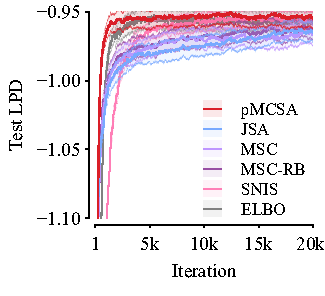
\includegraphics[scale=0.9]{figures/wine_01.pdf}
  }\hspace{0.2in}
  \subfloat[Wine]{
    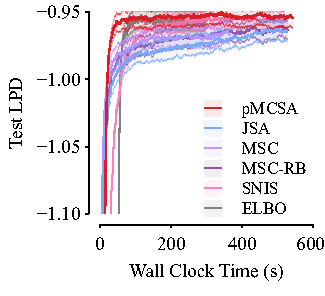
\includegraphics[scale=0.9]{figures/wine_02.pdf}
  } \\
  \subfloat[Concrete]{
    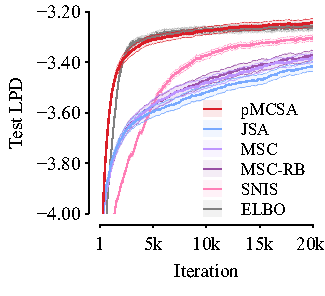
\includegraphics[scale=0.9]{figures/concrete_01.pdf}
  } \hspace{0.2in}
  \subfloat[Concrete]{
    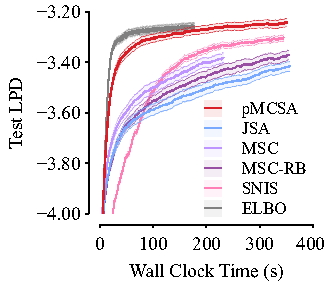
\includegraphics[scale=0.9]{figures/concrete_02.pdf}
  } \\
  \subfloat[Boston]{
    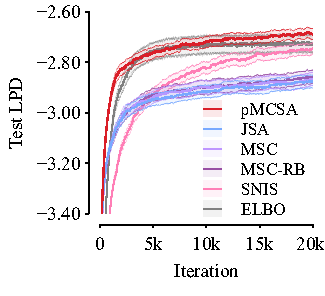
\includegraphics[scale=0.9]{figures/boston_01.pdf}
  }\hspace{0.2in}
  \subfloat[Boston]{
    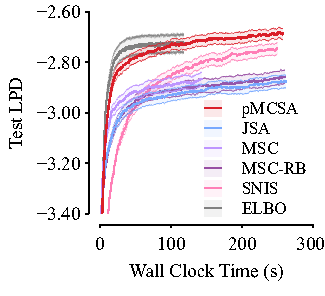
\includegraphics[scale=0.9]{figures/boston_02.pdf}
  } \\
  \subfloat[Yacht]{
    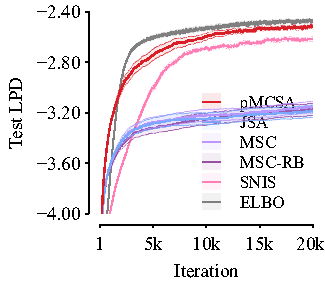
\includegraphics[scale=0.9]{figures/yacht_01.pdf}
  }\hspace{0.2in}
  \subfloat[Yacht]{
    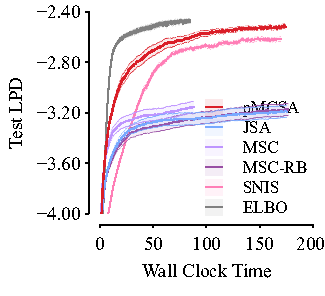
\includegraphics[scale=0.9]{figures/yacht_02.pdf}
  }
  \caption{Bayesian Neural Network Regression}
\end{figure}

%%% Local Variables:
%%% TeX-master: "master"
%%% End:


\end{document}
